\documentclass[conference]{IEEEtran}
\IEEEoverridecommandlockouts
% The preceding line is only needed to identify funding in the first footnote. If that is unneeded, please comment it out.
\usepackage[utf8]{inputenc}
\usepackage[english]{babel}
\usepackage{cite}
\usepackage{amsmath,amssymb,amsfonts}
\usepackage{physics}
\usepackage{dsfont}
\usepackage{algorithmic}
\usepackage{graphicx}
\usepackage{subcaption}
\usepackage{array}
\usepackage{float}
\usepackage{lipsum}
\usepackage{textcomp}
\usepackage{xcolor}

\usepackage[hidelinks]{hyperref}
\def\BibTeX{{\rm B\kern-.05em{\sc i\kern-.025em b}\kern-.08em
    T\kern-.1667em\lower.7ex\hbox{E}\kern-.125emX}}
\begin{document}

\title{Linear Analysis of Rössler System based on Circuits\\}

\author{\IEEEauthorblockN{Juan S. C\'ardenas R.}
\IEEEauthorblockA{\textit{Student} \\
\textit{Universidad EAFIT}\\
Medell\'in, Colombia\\
jscardenar@eafit.edu.co}
\and
\IEEEauthorblockN{David Plazas E.}
\IEEEauthorblockA{\textit{Student} \\
\textit{Universidad EAFIT}\\
Medell\'in, Colombia \\
dplazas@eafit.edu.co}
}

\maketitle

\begin{abstract}
In this work, the Rössler system is studied: a short introduction about the history of the system is given, as well as some state-of-the-art applications; a circuit implementation is presented based on the literature and translated to a state equation. The first part of this document is focused on give some basic theory, concepts and procedures to make a successful analysis of a linear system, which are applied and presented in the results section: a preliminary validation of the linear system obtained is performed making a comparison with the original Rössler system and an stability analysis is performed based on transfer functions and Bode diagrams. The simulations and the findings showed that the linear system in the selected operation point is stable, likewise intervals for one of the parameters that make the nonlinear and linear model stable as well; furthermore, the closed-loop stability was analyzed and properly validated. A linear approximation to Rössler equations was found with success (under some conditions).
\end{abstract}

\begin{IEEEkeywords}
Rössler system, simulation, state equation, dynamic system, transfer function, Bode diagram, stability analysis, linearization, order reduction, discrete dynamics, non-minimum phase system.
\end{IEEEkeywords}

\section{Introduction}
The system in study was proposed by O.E. R\"ossler  in 1976, as a simplified model with shape and behavior similar to spirals in Lorenz system, which was not fully understood at the time due to the techniques known to study oscillators were not applicable to Lorenz model \cite{rossler1976equation}. The R\"ossler equations are:

\begin{equation}
	\begin{array}{ll}
            \dot{x}&=-y-z\\
            \dot{y}&=x+ay\\
            \dot{z}&=b+z\left(x-c\right)
    \end{array}
\end{equation}

Although R\"ossler affirmed that the system did not have immediate physical interpretation \cite{rossler1976equation}, nowadays some applications can be found using the model as a mechanism and not as an abstraction of a physical system. The model presented has been used as a tool for image cryptography as it was shown by Mandal \textit{et al.} in  \cite{mandal2014symmetric}; in further work, Laiphrakpam and Khumanthem proposed improvements to Mandal's algorithm, as it is shown in \cite{laiphrakpam2017cryptanalysis}. On the other hand, coupled R\"ossler system with different inputs have been used to measure the correlation of time series, as Weule \textit{et al.} showed in \cite{weule1998detection}.

In order to bring the system to the real world, R\"ossler equations can be represented by a circuit, as Canals \textit{et al.} show in \cite{canals2014random}. The proposed circuit is shown in Fig. \ref{fig:circuito} and can be translated to 
\begin{equation}
	\begin{array}{ll}
            RC\dot{x}&=-y-z\\
            RC\dot{y}&=x+ay\\
            RC\dot{z}&=b+z\left(x-c\right)
    \end{array}\quad\quad\begin{array}{ll}
            a &= \dfrac{100k\Omega}{R_a}\vspace{2.5mm}\\
            b &= V_{cc}\dfrac{100k\Omega}{R_b}\vspace{2.5mm}\\
            c &= \dfrac{100k\Omega}{R_c}
    \end{array}\label{eq:circ}
\end{equation}
In \cite{canals2014random} they use this circuit to generate true random numbers using the output of the voltage of the node $z$. The nodes $x$ and $y$ have a fixed frequency of oscillation if the other variable is set to 0, since their rate of change are linear. In contrast, $z$ induces chaos to the circuit, due to its nonlinear behavior. In this manner, this variable was selected to be the output as its chaotic behavior is useful to generate random numbers \cite{canals2014random}.

In previous work \cite{JS_PL}, it was found that the Rössler system is stable for large input values. Based on this, it will be attempted to analyze this system as a linear model.

In this work, the question ``which linear model can successfully represent the Rössler circuit for certain input and parameters?''. It is difficult to give a hypothetical model without prior linear analysis, although it is believed that this model to be found will represent the system behavior, at least, in stationary state.

In order to achieve this, this work will begin linearizing the system in an equilibrium point, comparing the time response for both systems, close and far away from the operation point. Then, the respective continuous and discrete transfer function will be obtained and compared with the continuous linear model. It will be attempted to reduce the model's order using both analytic and software methods and compare this models with the linearized Rössler system; on the other hand, an stability analysis will be performed, using Ruth-Hurwitz criteria and root locus method. Finally a frequency response analysis will be performed using Bode diagrams of the original linearized model and the reduced ones; based on the Bode diagram for the linearized system, the closed-loop stability will be determined using phase and gain margins.

In section \ref{sec:meth}, the dynamic system used and some theory required to make the linear analysis of the Rössler system can be found. In section \ref{sec:results}, the results of every procedure are presented and applied to the Rössler system. In section \ref{sec:resultAn}, the analysis of the obtained results and their justification is made. Finally, the conclusions are presented in section \ref{sec:conc}.

%PREGUNTA INV; OBJETIVOS; TABLA CONTENIDOS, Etc.
\begin{figure*}
    \centering
    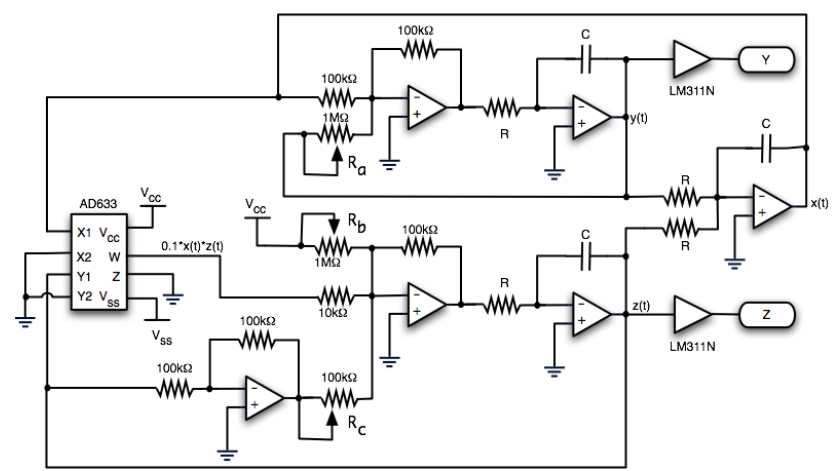
\includegraphics[scale=0.325]{figs/Circuito.png}
    \caption{R\"ossler circuit representation \cite{canals2014random}.}
    \label{fig:circuito}
\end{figure*}
\section{Methods}\label{sec:meth}
\subsection{Dynamic System}
In the circuit presented, according to Canals \textit{et al.} \cite{canals2014random}, the variables $x$, $y$ and $z$ represent the voltages through the nodes shown in Fig. \ref{fig:circuito}. The $RC$ parameter defines the system's time (in seconds), the supplied voltages are $V_{cc}=15V$ and $V_{ss}=-15V$; $R_a$, $R_b$ y $R_c$ are resistors in $k\Omega$ used to calculate the system's original parameters, as shown in (\ref{eq:circ}).

The circuit can be represented through a dynamic equation, as follows:
\begin{equation}
\begin{cases}
	\dot{x_1}=\dfrac{1}{RC}\left(-x_2-x_3\right)&\vspace{2mm}\\\vspace{2mm}
	\dot{x_2}=\dfrac{1}{RC}\left(x_1+\dfrac{100k\Omega}{R_a}x_2\right)&\\
	\dot{x_3}=\dfrac{1}{RC}\left[\left(V_{cc0}+u\left(t\right)\right)\dfrac{100k\Omega}{R_b}+x_3\left(x_1-\dfrac{100k\Omega}{R_c}\right)\right]&\\
	y = x_3
\end{cases}
\label{eq:state}
\end{equation}
where $y$ is the output and $u$ the input; note that the parameter $V_{cc}$ was selected as input, based on equation (\ref{eq:circ}), thus we select an initial value $V_{cc0}$ and add the input $u\left(t\right)$ in Volts. For the rest of this document, the state variable $x_3$ can sometimes be referred as $y$, since it has been chosen as the output.

\subsection{Simulation Diagram}
Using equation system (\ref{eq:state}), a simulation diagram was constructed using \textit{Simulink}, as Fig. \ref{fig:simulink} shows.
\begin{figure}
    \centering
    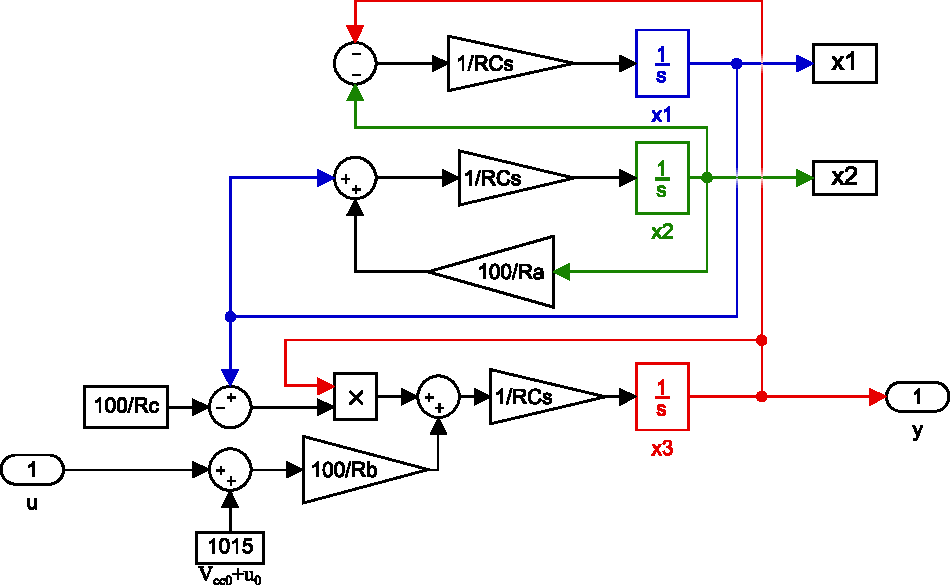
\includegraphics[scale=0.55]{figs/simulink.pdf}
    \caption{Simulation diagram for R\"ossler system.}
    \label{fig:simulink}
\end{figure}

\subsection{Linearity Curve}
The linearity curve is a tool that helps determine the range where the linear system can provide a suitable approximation to the stable nonlinear system. The linearity curve is obtained by simulating an stable system and registering the final value (stationary state) for a constant input, then the input is increased in a constant factor and then simulated until a new final value is found and so forth.

For the system in study, the following simulation diagram (Fig. \ref{fig:linearitySimulink}) was constructed, using \textit{Simulink}, in order to obtain the desired curve. As this figure shows, both systems are simulated with the same input. This one begins with a clock that should represent a continuous ``ramp'' over time, which is first scaled by a factor of $2/10$ and then passes through a Zero-Order-Hold (ZOH). This ZOH ensures that the continuous ``ramp'' is transformed into a discrete one, i.e. a ``staircase'' input since the signal is retained with a sampling time of $T=100s$. This means that both systems are simulated for $100s$ with a \textbf{constant} input. After this, the ZOH passes a new constant signal, where each iteration of the ZOH increases the input by $20V$ (this explains why it is scaled by $2/10$). Note that the initial input value $1000V$ has been included in the nonlinear simulation diagram, as Fig. \ref{fig:simulink} shows.
\begin{figure}[H]
    \centering
    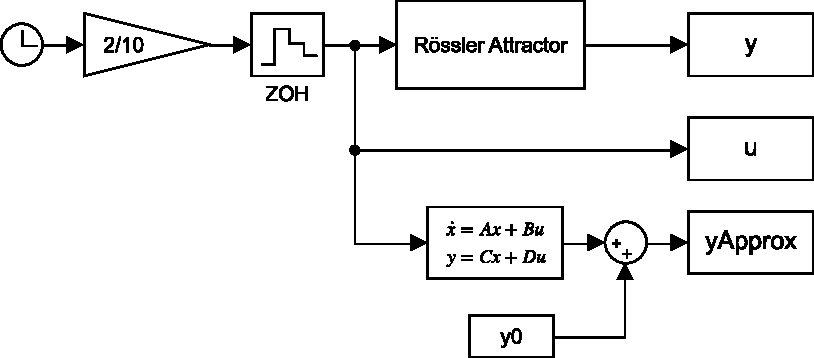
\includegraphics[scale=0.55]{figs/linearCurveSimulink.pdf}
    \caption{Simulation diagram for linearity curve.}
    \label{fig:linearitySimulink}
\end{figure}

\subsection{Linearization}
In order to linearize the system in study, the classical procedure will be performed. For more detailed notes on this method, see \cite[pp. 21-27]{antsaklis2007linear}. Given a nonlinear dynamic system
\begin{equation}
\begin{split}
    \mathbf{\dot{x}} =& f(\mathbf{x},\mathbf{u})\\
    \mathbf{y}=&g(\mathbf{x},\mathbf{u})
\end{split}
\end{equation}
We can obtain a linearization of this system around an operation point $(\mathbf{x_0},\mathbf{u_0})$, in the form
\begin{equation}\label{eq:stateLinear}
\begin{split}
    \Delta\mathbf{\dot{x}} =& \mathbf{A} \Delta\mathbf{x}+\mathbf{B}\Delta\mathbf{u}\\
    \Delta\mathbf{y}=&\mathbf{C}\Delta\mathbf{x}+\mathbf{D}\Delta\mathbf{u}
\end{split}
\end{equation}
Where $\Delta \mathbf{x}=\mathbf{x}-\mathbf{x_0}$, $\Delta \mathbf{u}=\mathbf{u}-\mathbf{u_0}$, $\Delta \mathbf{y}=\mathbf{y}-\mathbf{y_0}$; and $\mathbf{A}$, $\mathbf{B}$, $\mathbf{C}$ and $\mathbf{D}$ are Jacobians of the functions $f$ and $g$ as follows
\begin{equation}
\begin{split}
    \mathbf{A}=\dfrac{\partial f}{\partial\mathbf{x}}(\mathbf{x_0},\mathbf{u_0})&\qquad \mathbf{B}=\dfrac{\partial f}{\partial\mathbf{u}}(\mathbf{x_0},\mathbf{u_0})\\
    \mathbf{C}=\dfrac{\partial g}{\partial\mathbf{x}}(\mathbf{y_0},\mathbf{u_0})&\qquad \mathbf{D}=\dfrac{\partial g}{\partial\mathbf{u}}(\mathbf{y_0},\mathbf{u_0})
\end{split}
\end{equation}
This procedure can be also performed using \textit{Matlab}, through the command \texttt{linmod} with the following syntax: \texttt{[$\mathbf{A}$,$\mathbf{B}$,$\mathbf{C}$,$\mathbf{D}$] = linmod(\textit{sys},$\mathbf{x}_0$,$\mathbf{u}_0$)}, where \texttt{\textit{sys}} is a \textit{Simulink} model, and $(\mathbf{x}_0,\mathbf{u}_0)$ is the operation point.

\subsection{Linear and Nonlinear systems comparison}
As it has been already depicted, the linearization of a nonlinear model is given in $\Delta$-variables; in order to compare properly the output of a nonlinear system and its linearization, the scheme shown in Fig. \ref{fig:howto} can be used. Note that, for the linear system, is required to subtract the initial input $\mathbf{u_0}$ to obtain $\Delta\mathbf{u}$, and the output is given as $\Delta\mathbf{y}$, then the initial value $\mathbf{y_0}$ is added to obtain the standard output $\mathbf{y}(t)$
\begin{figure}[H]
    \centering
    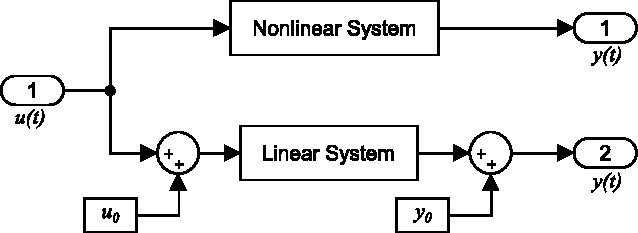
\includegraphics[scale=0.6]{figs/howtoLinearNonlinear.pdf}
    \caption{Diagram for comparing a nonlinear system with its linearization.}
    \label{fig:howto}
\end{figure}

\subsection{Transfer Function}\label{sec:tf}
The transfer function is a tool to represent a linear system with null initial conditions. For a single-input single-output (SISO) system, it is defined as the relation between the Laplace transform ($\mathcal{L}$) of the output and the Laplace transform of the input, as follows:
\begin{equation}
    G(s)=\dfrac{Y(s)}{U(s)}
\end{equation}
Where $Y(s)=\mathcal{L}\{y(t)\}$, $U(s)=\mathcal{L}\{u(t)\}$. For a discrete system, it would be worked with the $\mathcal{Z}$ transform. If the system is in a state-space representation, as in equation (\ref{eq:stateLinear}), the transfer function can be also obtained with
\begin{equation}\label{eq:ss2tf}
    G(s)=\mathbf{C}(s\mathbf{I}-\mathbf{A})^{-1}\mathbf{B}+\mathbf{D}
\end{equation}

And, finally, this can be achieved using \textit{Matlab}, using the command \texttt{tf(\textit{LinSys})}, where \texttt{\textit{LinSys}} is a linear system object (can be created with the command \texttt{ss($\mathbf{A}$,$\mathbf{B}$,$\mathbf{C}$,$\mathbf{D}$)}).

\subsection{Sampling Time}\label{sec:sampling}
The sampling time is a number that determines how often a continuous signal will be sampled in order to obtain a discrete signal.

In this work, the sample time was originally selected empirically, based on simulation: it was chosen such that the signal is sampled correctly (keeping oscillation period and most transitory behavior) and such that it can be easily evidenced the ``retained'' signal.

From a theoretical perspective, the sampling time can be obtained from the growth time ($T_r$) of the system in study. The growth time is defined at the time that the system takes to reach $90\%$ of stationary state from the respective $10\%$, and then apply the following criterion:
\begin{equation}
    \dfrac{T_r}{10}<T<\dfrac{T_r}{2}
\end{equation}
It is important to mention that the sample time selection is a non-trivial procedure, since a bad selection of the sample time can lead to undesired phenomena like the aliasing; for more information regarding the sample theorem and aliasing, refer to \cite[pp. 34-54]{diniz2010digital}. In this work, both methods are performed.

\subsection{Discretization of Transfer Functions}\label{sec:c2d}
Given a continuous transfer function $G(s)$, the discrete transfer function is obtained through the following expression:
\begin{equation}
    G(z)=(1-z^{-1})\mathcal{Z}\left\{\mathcal{L}^{-1}\left\{\dfrac{G(s)}{s}\right\}_{t\rightarrow kT}\right\}
\end{equation}
Where $T$ is a predefined sampling time for the discretization. This procedure can also be carried out using \textit{Matlab} with the command \texttt{c2d(\textit{transfer},T)} and, in this case, \texttt{\textit{transfer}} is a continuous transfer function.

\subsection{Ponderation Sequence}\label{sec:ponderationSequence}
The transfer function can be used to obtain a sequence of numbers that, given an input, the respective system output can be acquired. This numbers, in a continuous system, are infinite; thus, this sequence is often calculated for the discrete case.

Let $G(z)$ a discrete transfer function. The discrete ponderation sequence is found from the inverse $\mathcal{Z}$ transform of this transfer function:
\begin{equation}
    g(k)=\mathcal{Z}^{-1}\{G(z)\}
\end{equation}
And the output can be calculated with the following procedure:
\begin{equation}
    \begin{split}
        G(z)&=\dfrac{Y(z)}{U(z)}\\
        Y(z)&=G(z)U(z)\\
        \mathcal{Z}^{-1}\left\{Y(z)\right\}&=\mathcal{Z}^{-1}\left\{G(z)U(z)\right\}\\
        y(k)&=g(k)*u(k)
    \end{split}
\end{equation}
Where $*$ represent the convolution product, in this case, discrete.


\subsection{Order Reduction}\label{sec:reduct}
In order to reduce the system order, two straight-forward methods are often considered; this methods do not require formal procedures.

The first method is to cancel out stable zeros and poles that are close enough to each other and add a gain to assure that the stationary state for both systems is equal. The second method is to cancel out stable poles that are far enough from the dominant pole (at least 10 times the dominant pole) and, as the previous method, add a gain to compensate for the reduction.

On the other hand, in order to reduce the system order with more formal methods, \textit{Matlab} has the command \texttt{balred(\textit{Linear},\textit{order})}, where \texttt{\textit{Linear}} is an state-space model \textbf{or} a transfer function, and \texttt{\textit{order}} is the desired order after the reduction.

\textbf{2nd order approximation:\\} This method is a slightly more empirical/experimental approach. This method is based on the general formula for 2nd order transfer functions:
\begin{equation}
    G(s)=\dfrac{k\omega^2_0e^{-s\tau}}{s^2+2\zeta\omega_0s+\omega_0^2}
\end{equation}
Where $\omega_0$ is the natural frequency of the system, $\zeta$ is the damping, $k$ is the gain and $\tau$ is the delay. An example is shown in Fig. \ref{fig:example2ndOrder}.
\begin{figure}[H]
    \centering
    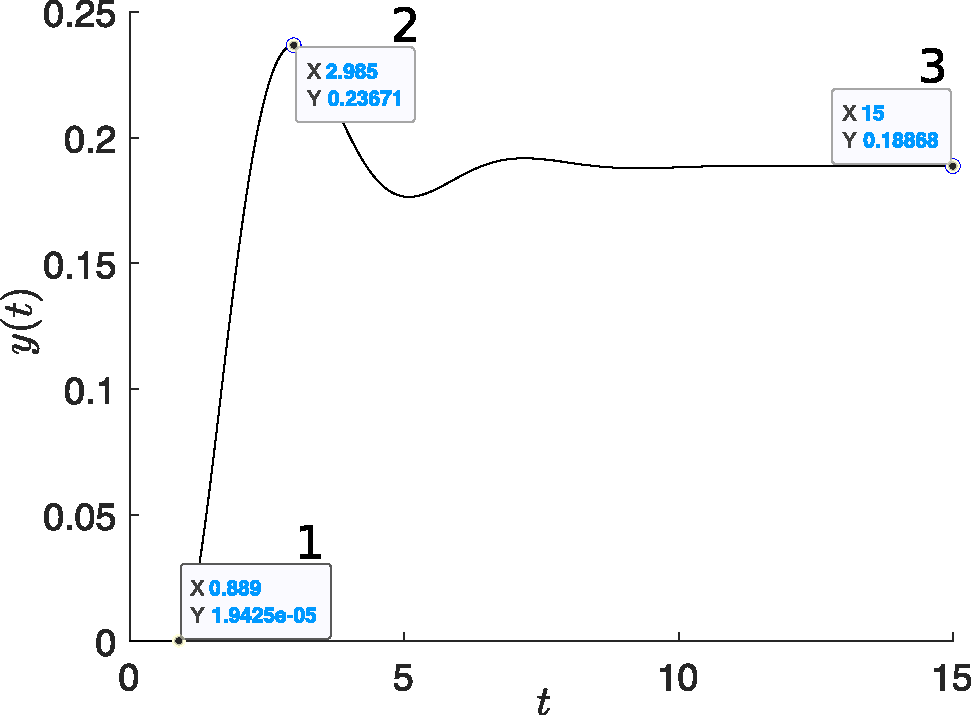
\includegraphics[scale=0.4]{figs/sis2ndOrder.pdf}
    \caption{Second order system.}
    \label{fig:example2ndOrder}
\end{figure}
In order to calculate the parameters, points 1, 2 and 3 are required. The first point gives information about the delay $\tau$, the second has information about the peak time $t_p$ and magnitude $y_p$. Finally, the last one shows the final value $y_{ss}$ (stationary state) and is needed to calculate the gain.

The following expression is used to calculate $\zeta$:
\begin{equation}
    \zeta=\dfrac{1}{\sqrt{1+\left(\dfrac{\pi}{\ln Mp}\right)^2}}
\end{equation}
Where
\begin{equation}
    Mp=\dfrac{y_p-y_{ss}}{y_{ss}}
\end{equation}
is the maximum overshoot; and through the following equation, $\omega_0$ is obtained:
\begin{equation}
    \omega_0=\dfrac{\pi}{t_p\sqrt{1-\zeta^2}}
\end{equation}

\subsection{Stability}
The following methods can only be applied to linear systems. For stability of nonlinear systems see reference \cite[Ch. 13]{dahleh2004lectures}, for Lyapunov stability.
\subsubsection{Poles Calculation}
The simplest way of knowing whether a linear system is stable is calculating all the poles $\lambda_i$ and checking if $\Re(\lambda_i)<0$. In \textit{Matlab}, the poles can be calculated directly from the state-space model or transfer function with the command \texttt{pole(\textit{Linear})}.

\subsubsection{Bounded-Input Bounded-Output Criterion (BIBO)}
Another way to determine if a linear system is stable is through the BIBO criterion \cite[Pag. 170]{antsaklis2007linear}: a bounded input (e.g. bounded waves, step, impulse train, etc.) generates a bounded output. It is important to highlight that this criterion does not necessarily imply that for every bounded input, the output will be bounded, but at least, for sine inputs. Another note is that this method is specially important when poles are exclusively imaginary ($\Re(\lambda_i)=0$).

\subsubsection{Routh-Hurwitz Method}
The Routh-Hurwitz method works with the characteristic polynomial of a linear system, that can be obtained from the denominator of the transfer function or with $P(s)=|s\mathbf{I}-\mathbf{A}|=0$.

Consider the general case:
\begin{equation}
    P(s)=\sum_{j=0}^na_js^{n-j}\quad a_0\neq0
\end{equation}
\textbf{Necessary Conditions:}
\begin{itemize}
    \item $(\forall j)(a_j>0)$
\end{itemize}
\textbf{Sufficient Conditions:}
\begin{itemize}
    \item The first column of the Routh-Hurwitz array is non-negative.
\end{itemize}

For a more detailed explanation of the Routh-Hurwitz array, refer to \cite[pp. 212-214]{ogata2010modern}. In \textit{Matlab}, an implementation has been developed and can be found in \cite{RHCaliche}.

\subsection{Root Locus}\label{sec:root_locus}
The root locus is a plot of how the roots of a polynomial change for a parameter $k>0$. It uses a closed-loop transfer function with a gain $k$ that is equivalent to this polynomial.

Given a polynomial with the parameter $k$ in one or more coefficients of the polynomial, it can always be expressed as 
\begin{equation}
    1+k\dfrac{N(s)}{D(s)}=0
\end{equation}
Note that this can be interpreted as a denominator of a closed-loop transfer function. Thus, the associated plant is 
\begin{equation}
    G(s)=\dfrac{N(s)}{D(s)}
\end{equation}

The root locus starts ($k=0$) in the poles of $G(s)$ and finishes ($k\rightarrow\infty$) in the finite and infinite zeros of $G(s)$. The root locus is useful to determine ranges of $k$ where the system associated with the characteristic polynomial $P(s)$ is stable. This procedure can also be used to determine the infinite zeros of a transfer function. The root locus can be obtained as well using \textit{Matlab} using \texttt{rlocus(\textit{Linear})}, where \texttt{\textit{Linear}} is a state-space model or a transfer function.

\subsection{Bode Diagram}\label{sec:bode}
The Bode diagram is a tool to analyze the frequency response. The frequency response is useful to analyze the system output when the input is a sine wave, since the output in stationary state will be another sine wave with equal frequency and different amplitude and phase.

The bode diagram is composed of two plots in logarithmic scale, since it is often desired to analyzed the frequency response for a wide spectrum of frequencies: one for the relative amplitude and another one for the phase of the output (in stationary state). For the amplitude, it is given in decibels (dB) and for the phase, it is given in degrees.

Suppose the input is
\begin{equation}
    u(t)=A\sin(\omega t)
\end{equation}
And the output in stationary state
\begin{equation}
    y_{ss}(t)=B\sin(\omega t+\phi)
\end{equation}
It can be proved (see \cite[pp. 399-400]{ogata2010modern}) that \[B=A|G(i\omega)|\]\[\phi=\arctan\left(\dfrac{\Im[G(i\omega)]}{\Re[G(i\omega)]}\right)\] And the amplitude in decibels is defined as 
\begin{equation}
    |G(i\omega)|\text{dB}=20\log_{10}\left(\dfrac{B}{A}\right)
\end{equation}
The Bode diagram is useful for several reasons. In first place, it can be used to determine the regions where the system intensifies or reduces the input amplitude. On the other hand, it can be used to determine the ranges of gain and delay where the closed-loop system is stable. Lastly, it can help determine whether the system in study is a minimum phase system.

The bode diagram can be obtained using \textit{Matlab} through the command \texttt{bode(\textit{Linear})}, where \texttt{\textit{Linear}} is a transfer function or a linear state-space model.

As it was previously mentioned, the Bode diagram can be used to determine closed-loop stability, using the phase and gain margins. For a more detailed explanation regarding the phase and gain margins see \cite[pp. 464-468]{ogata2010modern}. With \textit{Matlab}, the margins can be calculated with the command \texttt{allmargin(\textit{Linear})}, where Linear is a state-space model or a transfer function.



\section{Results}\label{sec:result}
All the following simulations were implemented in Simulink, using fourth order Runge-Kutta algorithm with fixed step size of $0.001$.
\subsection{Model Validation}
Before proceeding with further analysis, the model in analysis must be tested and compared with known results.

The comparison will be done with 2 different authors. First, R\"ossler original paper \cite[Fig. 2]{rossler1976equation} will be used as reference. R\"ossler firstly proposed the model using $a=b=0.2$ and $c=5.7$ with initial conditions $(x_{10},x_{20},y_{0})=(0,-6.78,0.02)$.
Thus, the parameters for our circuit simulation will be $u(t)=0V$, $V_{cc0}=15V$, $RC=1s$, $R_a=500k\Omega$, $R_b=7500k\Omega$, $R_c=17.5934k\Omega$, with $t_0=0s$ and $t_{\text{end}}=339.249s$. The results of the simulation are shown in Fig. \ref{fig:validRoss}.

\begin{figure}[H]
    \centering
    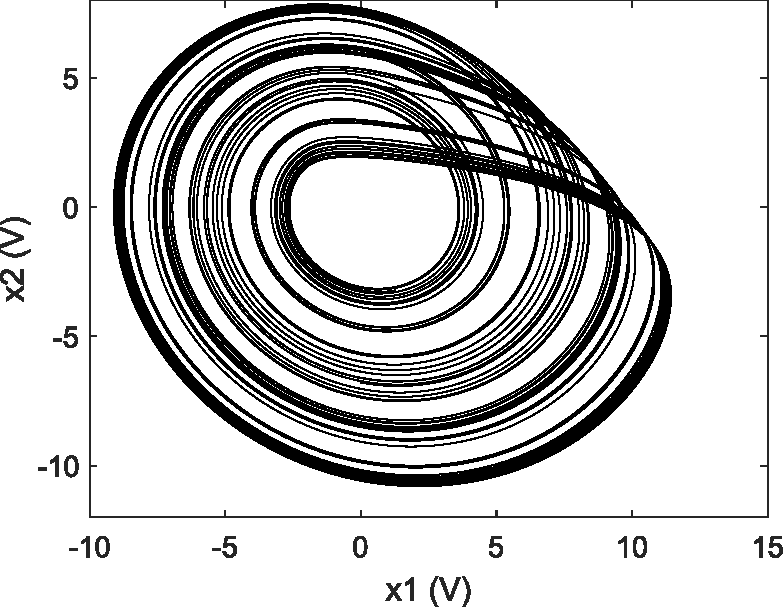
\includegraphics[scale=0.4]{figs/x1vsx2ValidRoss.pdf}
    \caption{Phase portrait results of $x_2x_1$ plane using R\"ossler \cite{rossler1976equation} parameters.}
    \label{fig:validRoss}
\end{figure}

This figure shows the trajectory followed by the system between $t=0$ and $t=339.249$, note that it follows an enclosed trajectory but not necessarily periodic; note as well the Möbius strip-like behavior, as Rössler states in his main paper \cite{rossler1976equation}.

On the other hand, Sprott and Li presented useful simulations for R\"ossler system, providing results for both phase portraits and time responses of the state variables \cite[Figs. 2 and 3]{sprott2017asymmetric}. The simulations were done with $a=0.29$, $b=0.14$ and $c = 4.52$, with two initial conditions: $IC1 = (-1.25, -0.72, -0.10)$ and $IC2 = (0.72,1.28,0.21)$. Thus, our circuit parameters are $u(t)=0V$, $V_{cc0}=15V$, $RC=1s$, $R_a=344.8276k\Omega$, $R_b=10714k\Omega$, $R_c=22.1239k\Omega$, with $t_0=0s$ and $t_{\text{end}}=100s$.

The results for the phase portraits are shown in Fig. \ref{fig:validPhase} and for the time responses in Fig. \ref{fig:validTime}.
\begin{figure*}
        \centering
        \begin{subfigure}[b]{0.3\textwidth}
            \centering
            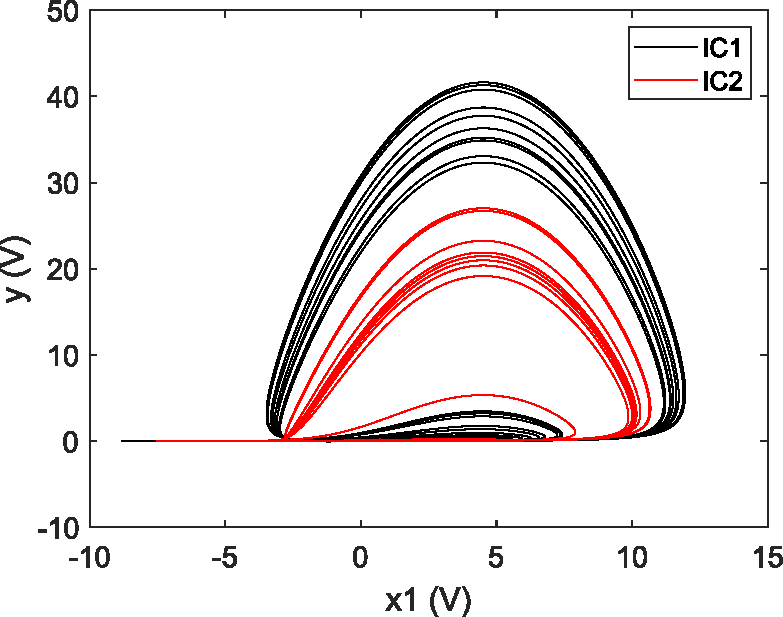
\includegraphics[scale=0.35]{figs/yvsx1Valid.pdf}
        \end{subfigure}
        \begin{subfigure}[b]{0.3\textwidth}  
            \centering 
            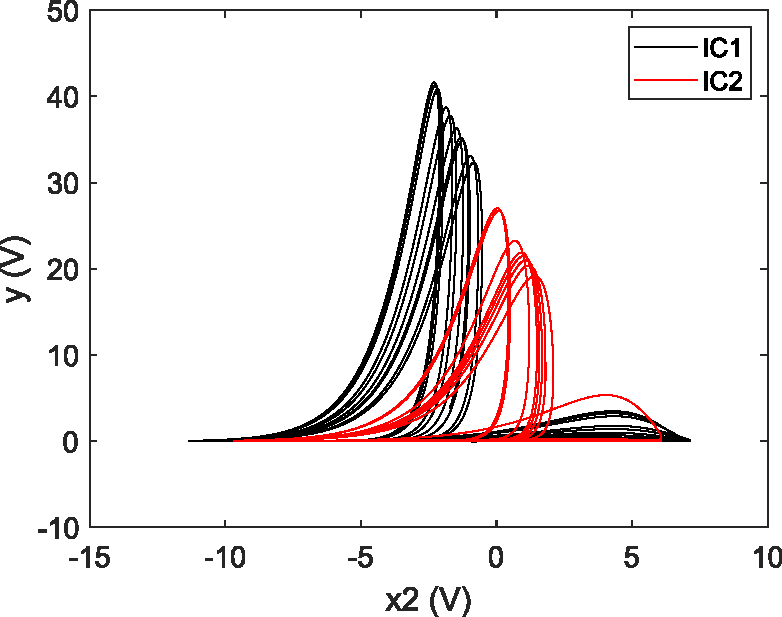
\includegraphics[scale=0.35]{figs/yvsx2Valid.pdf}
        \end{subfigure}
        \begin{subfigure}[b]{0.3\textwidth}   
            \centering 
            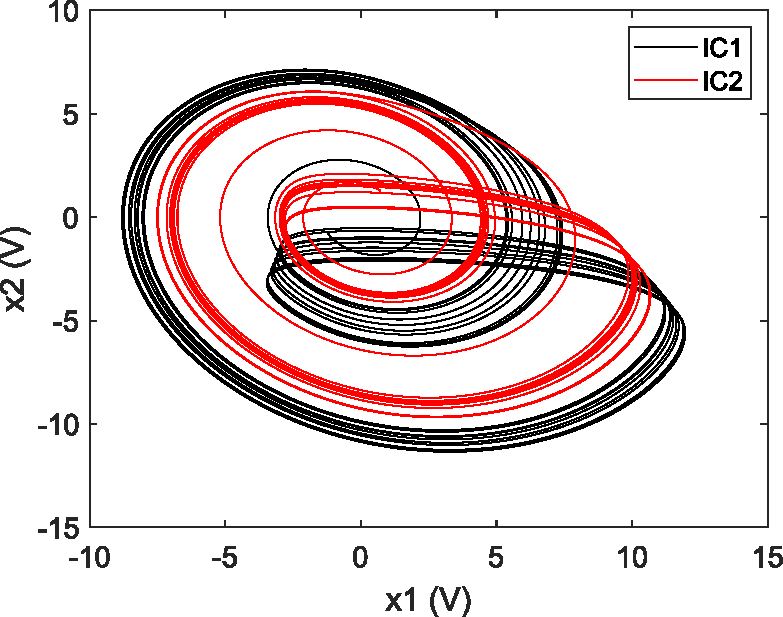
\includegraphics[scale=0.35]{figs/x2vsx1Valid.pdf}
        \end{subfigure}
        \caption{Phase portraits for the state variables with $IC1$ and $IC2$ as initial conditions.}
        \label{fig:validPhase}
	\end{figure*}

	\begin{figure*}
        \centering
        \begin{subfigure}[b]{0.3\textwidth}
            \centering
            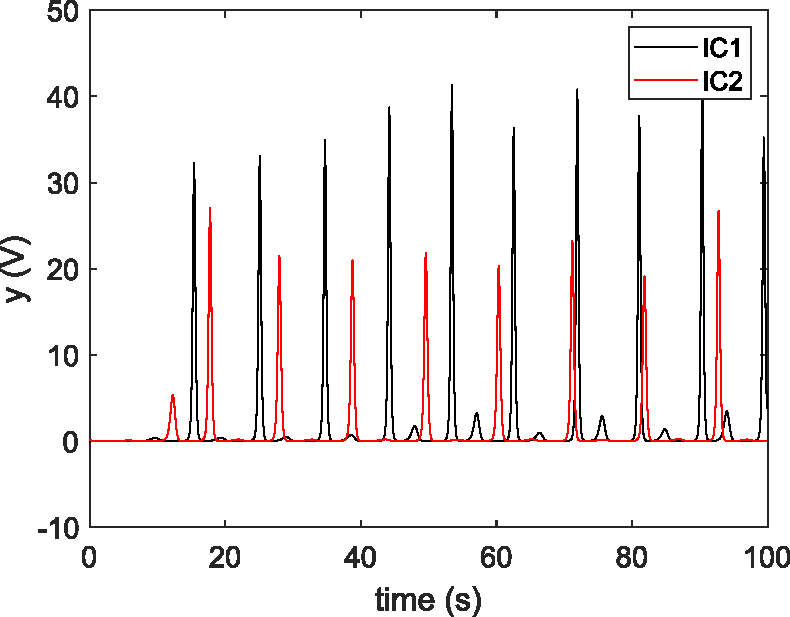
\includegraphics[scale=0.35]{figs/yvstValid.pdf}
        \end{subfigure}
        \begin{subfigure}[b]{0.3\textwidth}  
            \centering 
            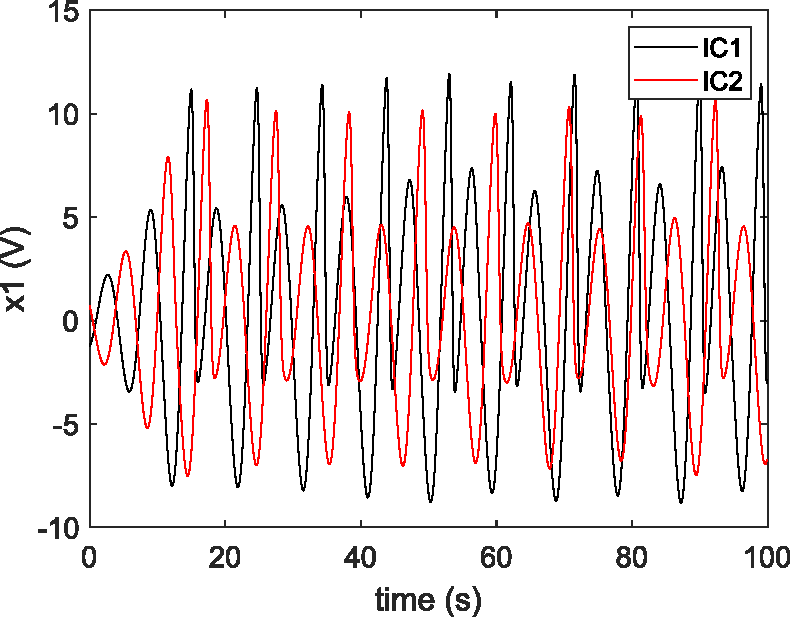
\includegraphics[scale=0.35]{figs/x1vstValid.pdf}
        \end{subfigure}
        \begin{subfigure}[b]{0.3\textwidth}   
            \centering 
            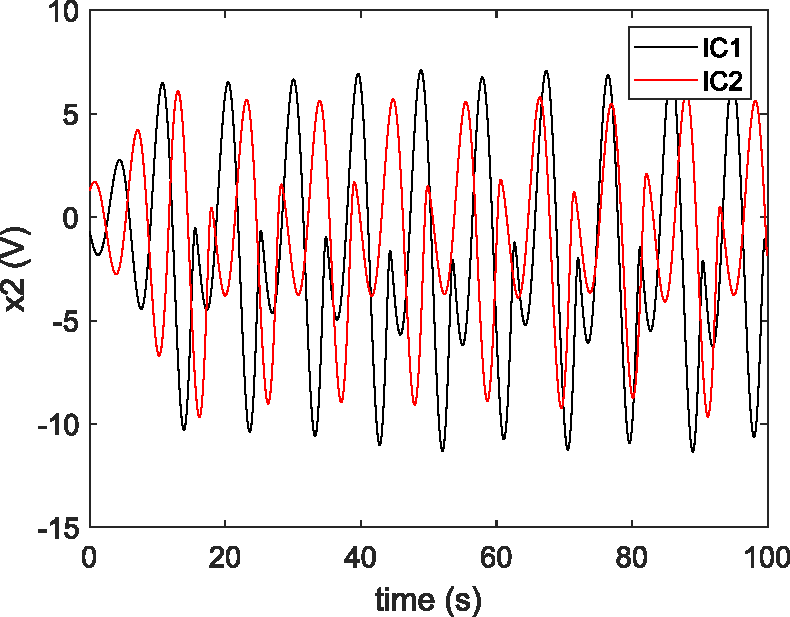
\includegraphics[scale=0.35]{figs/x2vstValid.pdf}
        \end{subfigure}
        \caption{Time responses for signals $y$, $x_1$, $x_2$ with initial conditions $IC1$ and $IC2$.}
        \label{fig:validTime}
	\end{figure*}
	%%%%%%%%%%%%%%%%%%%%%%%%%%%%%%%%%%%%%%%%%%%%%%%%%%%%%%%%%%%%%%%%%%%%%%%%%%%%%%
	\subsection{Input Variations}
	For comparing the results, we will be using the original R\"ossler model initialization \cite{rossler1976equation} as a reference and this simulation will be used for comparison. The parameters are $u(t)=0V$, $V_{cc0}=15V$, $RC=1s$, $R_a=500k\Omega$, $R_b=7500k\Omega$, $R_c=17.5439k\Omega$, with $t_0=0s$, $t_{\text{end}}=100s$ and initial conditions $(x_{10},x_{20},y_{0})=(0,-6.78,0.02)$. For all the following simulations, only the 3D plot for the state variables and the output response in time will be presented. In Figs. \ref{fig:3DRosslerO} and \ref{fig:RosslerO} the reference simulation results are presented. Three different inputs were selected according to our input definition: two sine waves and a step in the $V_{cc}$ voltage.
	
	\begin{figure}[H]
	    \centering
	    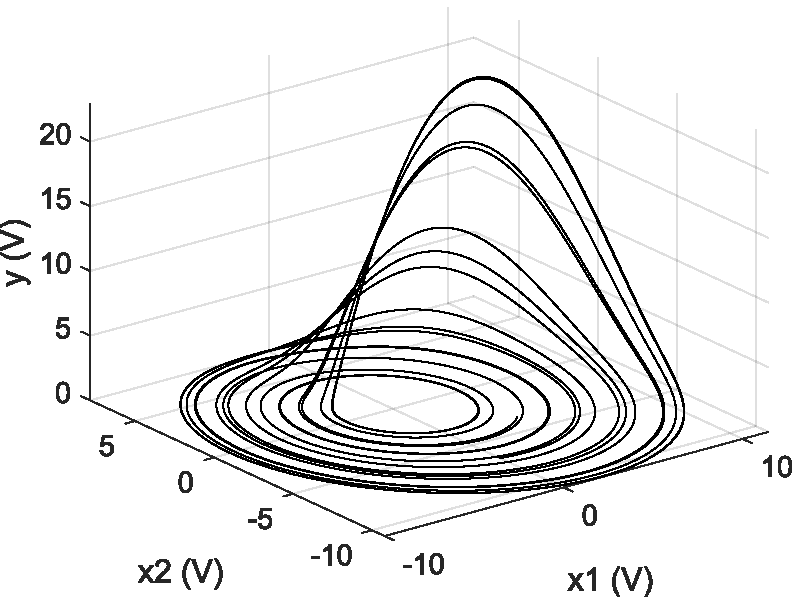
\includegraphics[scale=0.48]{figs/OriginalRosslerAttractor3d.pdf}
	    \caption{3D plot for the state variables and the output for reference Rössler attractor.}
	    \label{fig:3DRosslerO}
	\end{figure}
	\begin{figure}
	    \centering
	    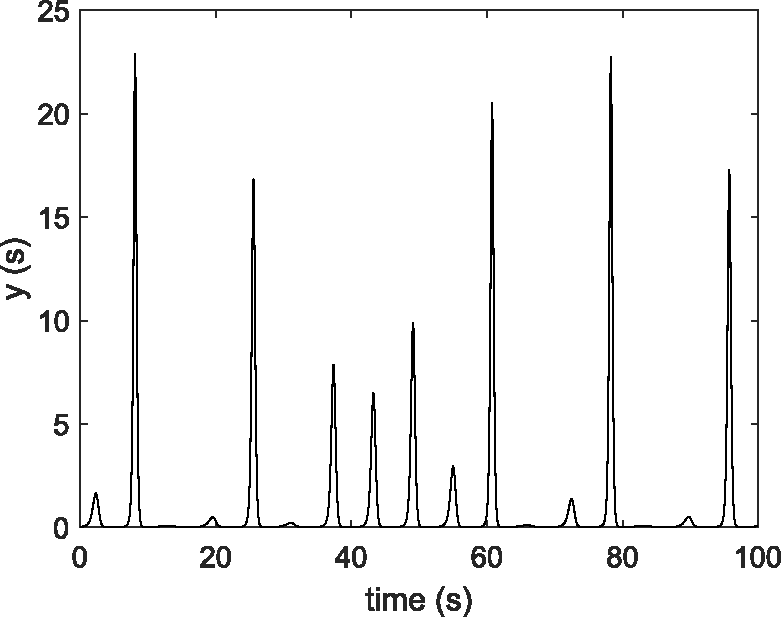
\includegraphics[scale=0.38]{figs/OriginalRosslery.pdf}
	    \caption{Output signal in time for reference Rössler attractor.}
	    \label{fig:RosslerO}
	\end{figure}
    It is important to highlight that the behavior showed in Fig. \ref{fig:RosslerO} is a good example of the response that Canals \textit{et al.} \cite{canals2014random} affirmed: the peaks in the output signal are unpredictable in time (this does not imply that the system is unpredictable).
	
    \subsubsection{Sines Inputs}\label{subsubsec:sines}
    First, a sine wave with frequency $\omega=2\text{rad}*s^{-1}$, amplitude $A=500V$ and offset of $b=500V$. Thus, the input is
    
    \begin{equation}
        u(t)=(500V)\sin({2t})+500V
    \end{equation}
    The plot for this input is shown in Fig. \ref{fig:inputSin2f}. The system's response is shown in Figs. \ref{fig:3dSin2f} and \ref{fig:OutSin2f}.
    \begin{figure}[H]
        \centering
        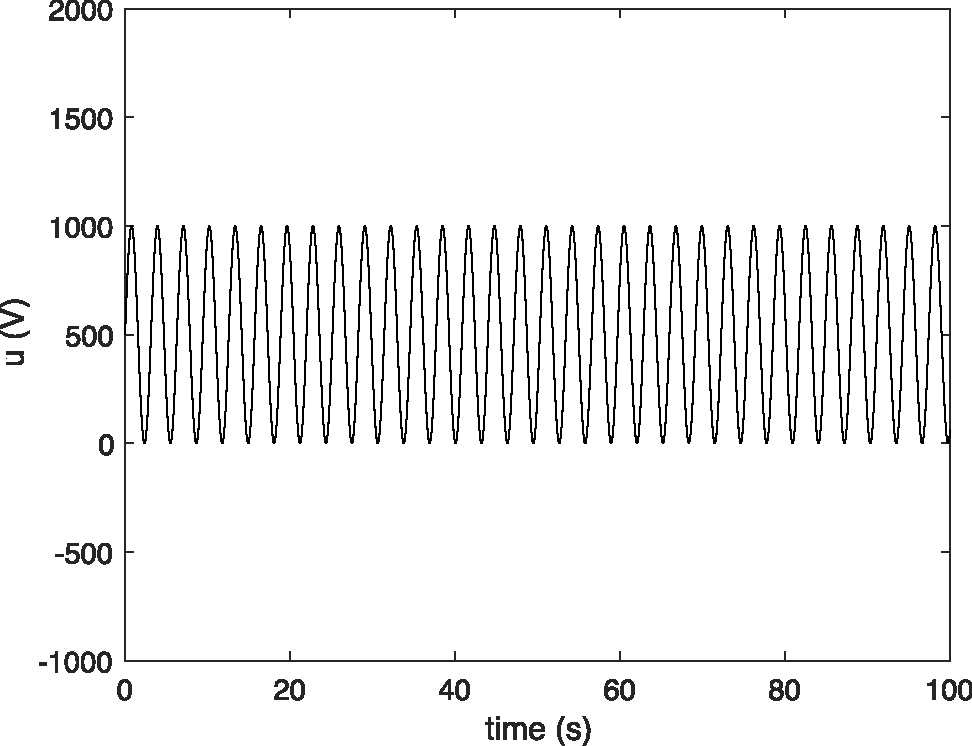
\includegraphics[scale=0.32]{figs/InputSin2f.pdf}
        \caption{Input sine wave with $\omega=2\text{rad}*s^{-1}$.}
        \label{fig:inputSin2f}
    \end{figure}
    \begin{figure}[H]
        \centering
        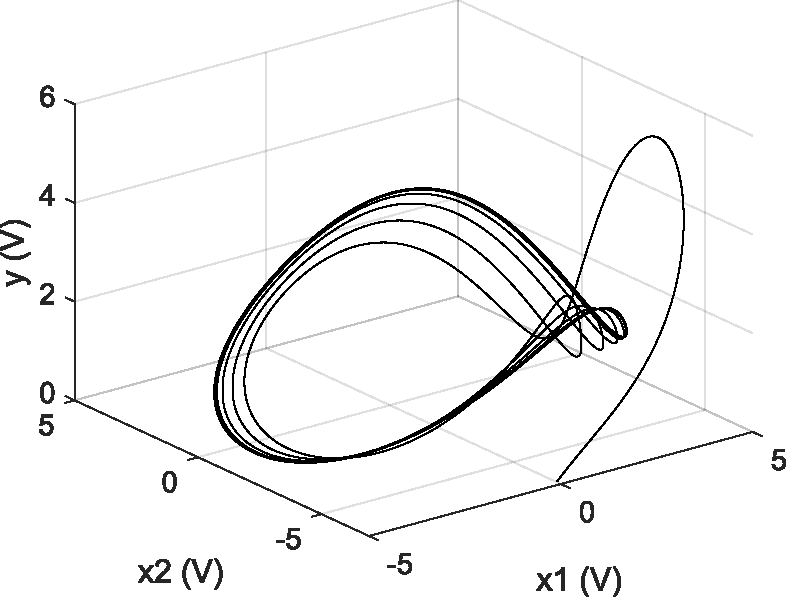
\includegraphics[scale=0.45]{figs/3dSine2fInput.pdf}
        \caption{Phase portrait for the three state variables with sine input.}
        \label{fig:3dSin2f}
    \end{figure}
    \begin{figure}[H]
        \centering
        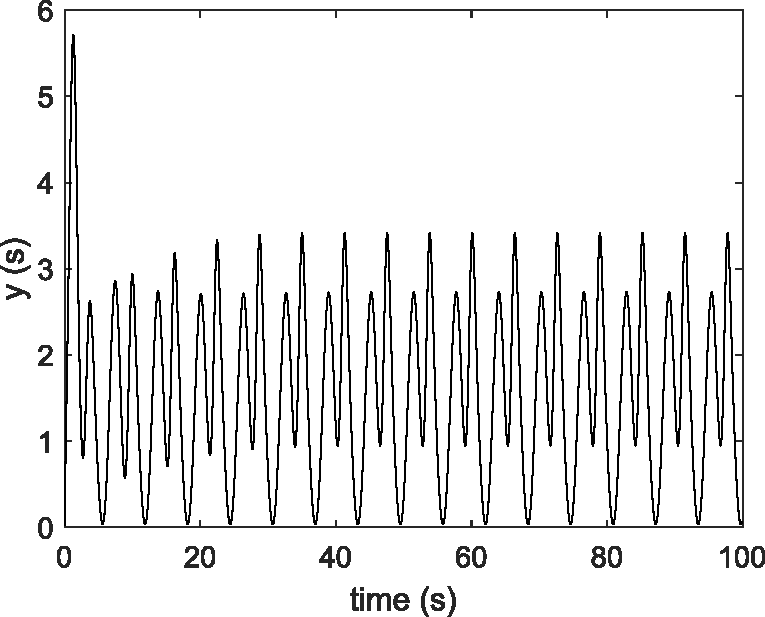
\includegraphics[scale=0.4]{figs/OutSine2fInput.pdf}
        \caption{Output signal response in time for sine input.}
        \label{fig:OutSin2f}
    \end{figure}
    
    Notice that eventually the trajectory falls in a closed and periodic orbit; as expected, the output signal is periodic but first modulated by an increasing signal.
    
    Second, a sine wave with frequency $\omega=5\text{rad}*s^{-1}$, amplitude $A=500V$ and offset of $b=500V$. Thus, the input is
    
    \begin{equation}
        u(t)=(500V)\sin({5t})+500V
    \end{equation}
    The plot for this input is shown in Fig. \ref{fig:inputSin5f}. The system's response is shown in Figs. \ref{fig:3dSin5f} and \ref{fig:OutSin5f}.
    
    \begin{figure}[H]
        \centering
        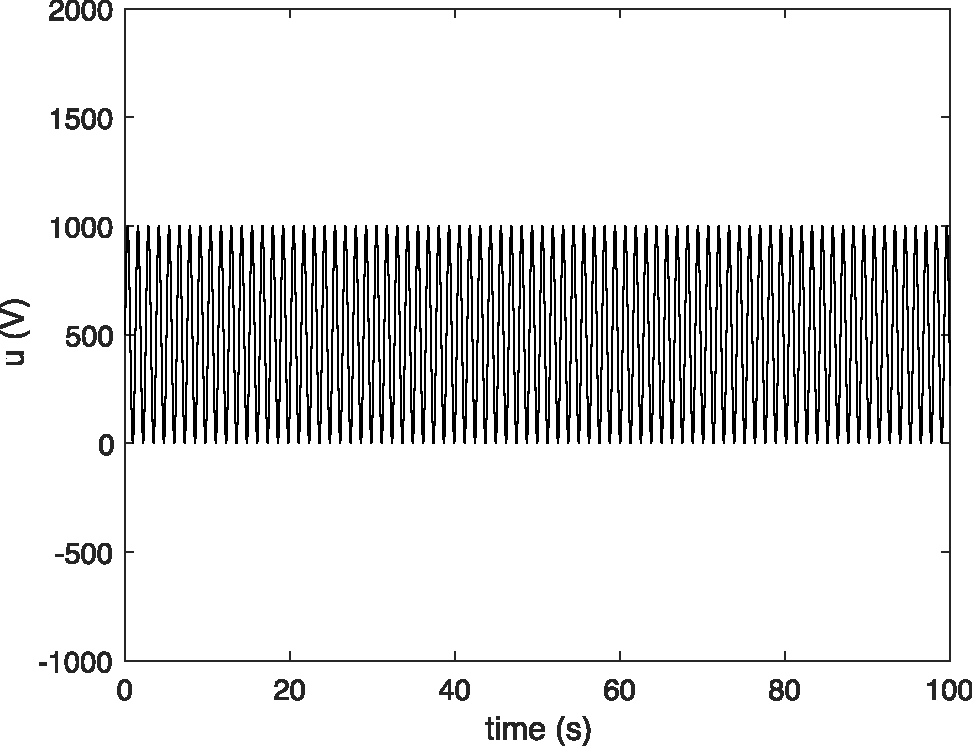
\includegraphics[scale=0.375]{figs/InputSin5f.pdf}
        \caption{Input sine wave with $\omega=5\text{rad}*s^{-1}$.}
        \label{fig:inputSin5f}
    \end{figure}
    \begin{figure}[H]
        \centering
        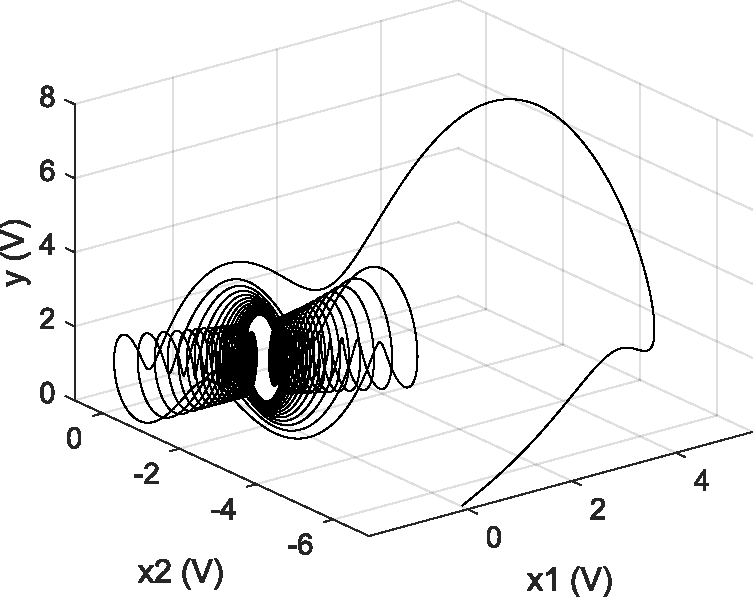
\includegraphics[scale=0.425]{figs/3dSine5fInput.pdf}
        \caption{Phase portrait for the three state variables with sine input.}
        \label{fig:3dSin5f}
    \end{figure}
    \begin{figure}[H]
        \centering
        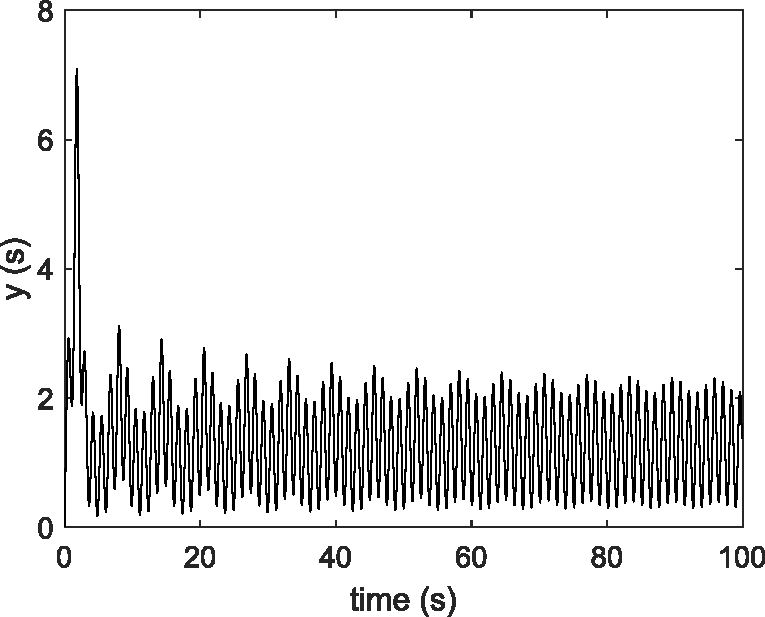
\includegraphics[scale=0.4]{figs/OutSine5fInput.pdf}
        \caption{Output signal response in time for sine input.}
        \label{fig:OutSin5f}
    \end{figure}
    
    As well as the previous sine input, the system falls into a periodic orbit that first decreases its amplitude. The output signal is periodic but modulated by a decreasing signal.
    
    \subsubsection{Step}\label{subsubsec:step}
    The step input was selected with step time of $40s$, initial value of $0V$ and final value of $1000V$. Hence, the input is given by
    
    \begin{equation}
        u(t)=(1000V)H(t-40s)
    \end{equation}
    Where $H(t)$ is the Heaviside step function. Fig. \ref{fig:inputStep} shows the step input and Figs. \ref{fig:3dStep} and \ref{fig:outStep} show the simulation results.
    \begin{figure}[H]
        \centering
        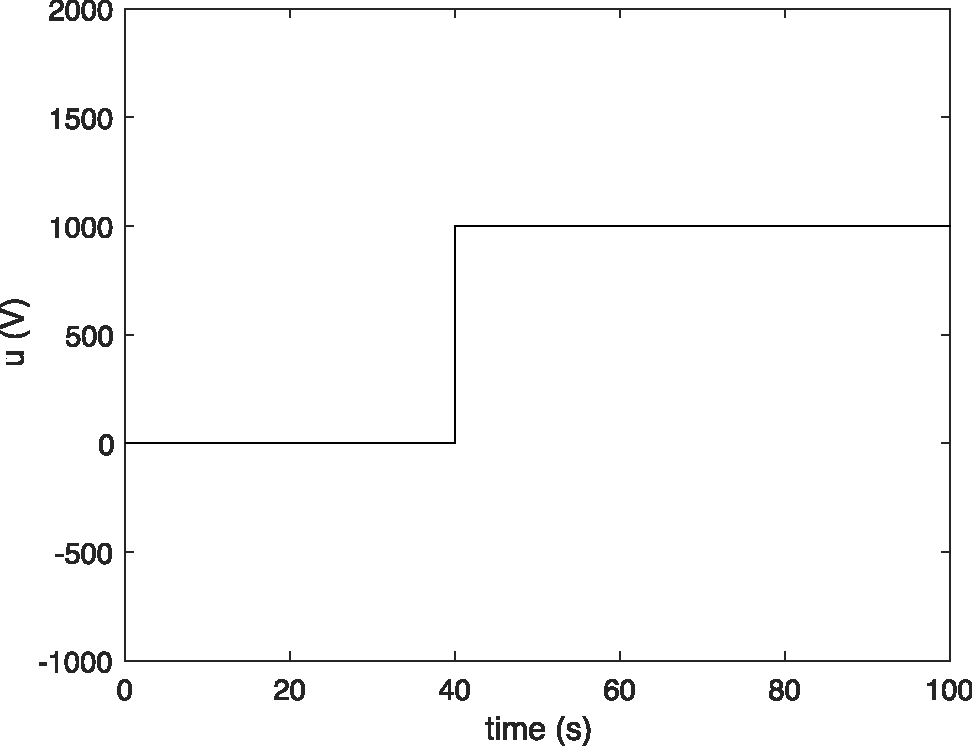
\includegraphics[scale=0.35]{figs/InputStep.pdf}
        \caption{Step input.}
        \label{fig:inputStep}
    \end{figure}
    \begin{figure}[H]
        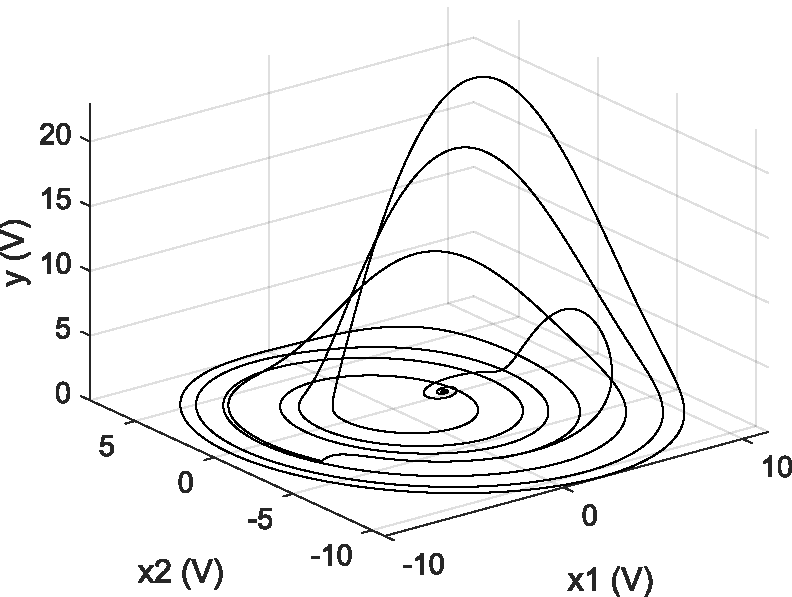
\includegraphics[scale=0.4]{figs/3dStepInput.pdf}
        \centering
        \caption{3D phase portrait for $x_1$, $x_2$ and $y$}
        \label{fig:3dStep}
    \end{figure}
    \begin{figure}[H]
        \centering
        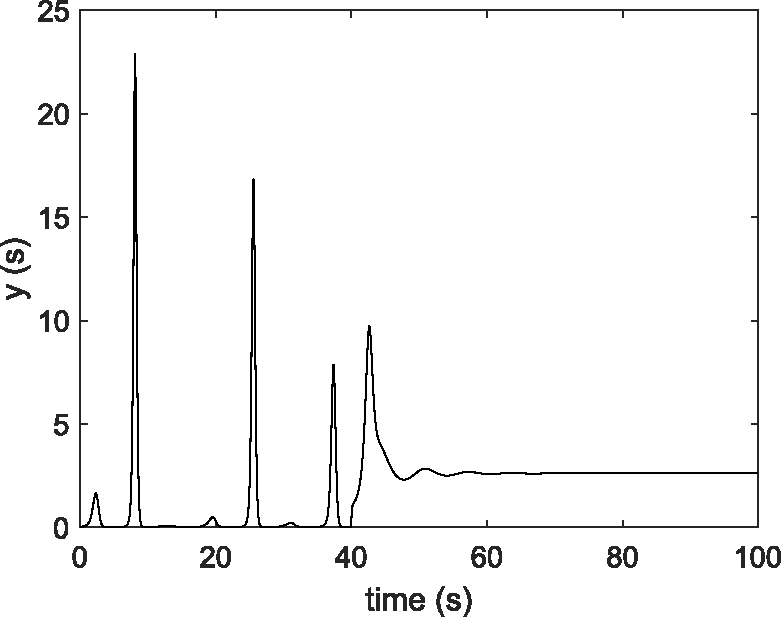
\includegraphics[scale=0.4]{figs/OutStepInput.pdf}
        \caption{Output signal response in time for step input.}
        \label{fig:outStep}
    \end{figure}
    
    The 3D plot for the state variables shows that it starts normally as the Rössler attractor, but once the input is applied, the system stabilizes in completely, converging to an specific point in space. In the output signal through time the stability is evidenced in the constant value for $y$. 
    
    %%%%%%%%%%%%%%%%%%%%%%%%%%%%%%%%%%%%%%%%%%%%%%%%%%%%%%%%%%%%%%%%%%%%%%%%%%%%%%
    \subsection{Parameter Variation}
    In this section, several simulations were made varying the values for parameters $R_a$ and $R_c$, choosing values with important impact in the system's response. All simulations were made assuming $u(t)=0V$, $V_{cc0}=15V$, $RC=1s$, $R_a=500k\Omega$, $R_b=7500k\Omega$, $R_c=17.5439k\Omega$, with $t_0=0s$, $t_{\text{end}}=100s$ and initial conditions $(x_{10},x_{20},y_{0})=(0,-6.78,0.02)$. Keep in mind that, when a parameter is selected to vary, the rest of the parameters, initial conditions and solution method remains the same.
    
    It is important to highlight that $R_b$ was not chosen for the parameter variation since varying it is similar to changing the input for the system.
    
    \subsubsection{Parameter \texorpdfstring{$R_a$}{Ra}}\label{subsubsec:varparaA}
    For parameter $R_a$, higher values from the reference $R_a=500k\Omega$ were selected, since smaller values than the reference produces behaviors similar enough with the reference system (Figs. \ref{fig:3DRosslerO} and \ref{fig:RosslerO}), even though there is a point where the response changes completely; this result will be presented in section \ref{subsubsec:ra}. The selected values for the parameter are $R_{a_1} = 650k\Omega$, $R_{a_2} = 750k\Omega$, $R_{a_3} = 1750k\Omega$ and $R_{a_4} = 3652k\Omega$. The results are shown in Figs. \ref{fig:3dparaAvar} and \ref{fig:paraAvar}.
    
    \begin{figure*}
        \centering
        \begin{subfigure}[b]{0.22\textwidth}
            \centering
            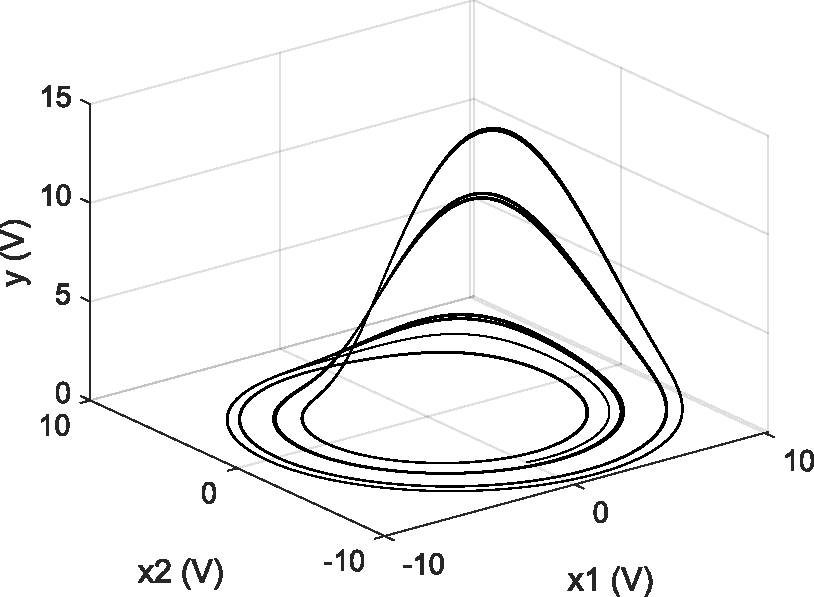
\includegraphics[scale=0.28]{figs/paraA/3dParaA650.pdf}
            \caption{$R_{a_1} = 650k\Omega$.}    
        \end{subfigure}
        \begin{subfigure}[b]{0.22\textwidth}  
            \centering 
            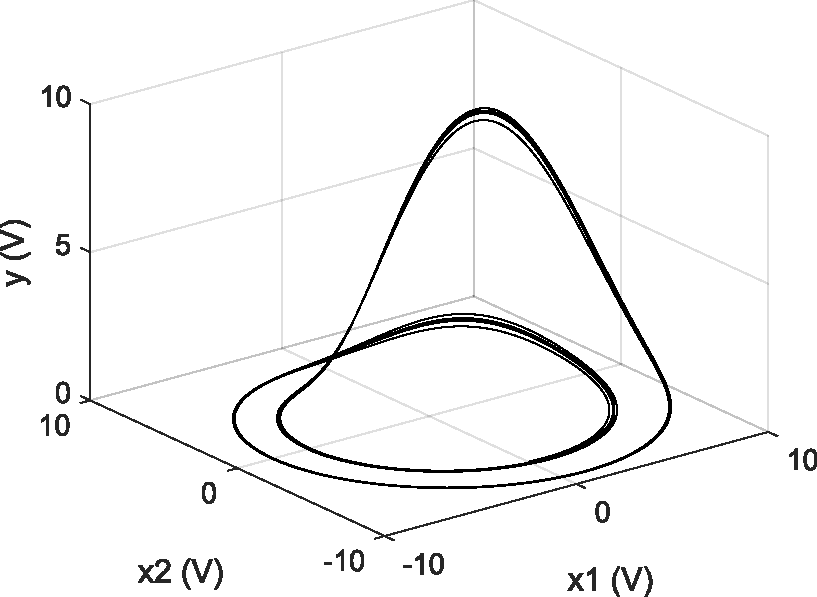
\includegraphics[scale=0.28]{figs/paraA/3dParaA750.pdf}
            \caption{$R_{a_2} = 750k\Omega$.}  
        \end{subfigure}
        \begin{subfigure}[b]{0.22\textwidth}   
            \centering 
            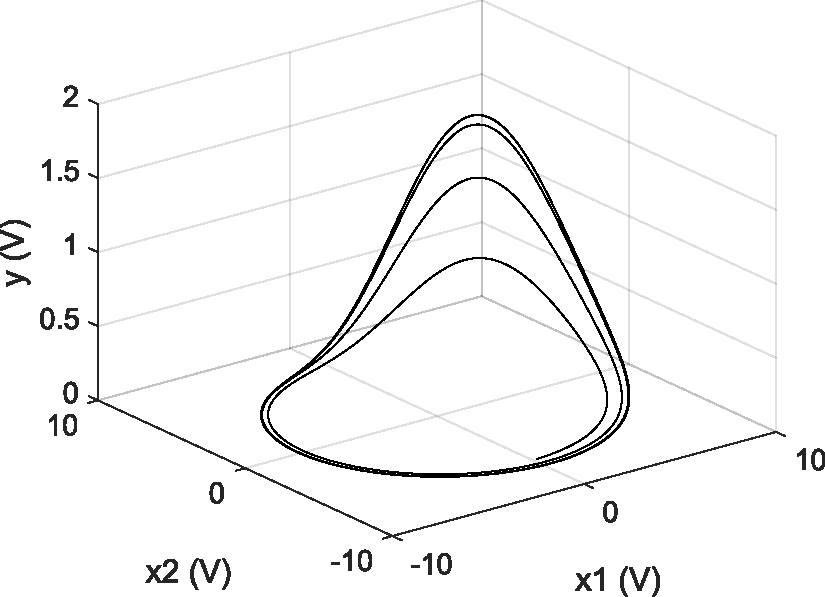
\includegraphics[scale=0.28]{figs/paraA/3dParaA1750.pdf}
            \caption{$R_{a_3} = 1750k\Omega$}    
        \end{subfigure}
        \begin{subfigure}[b]{0.22\textwidth}   
            \centering 
            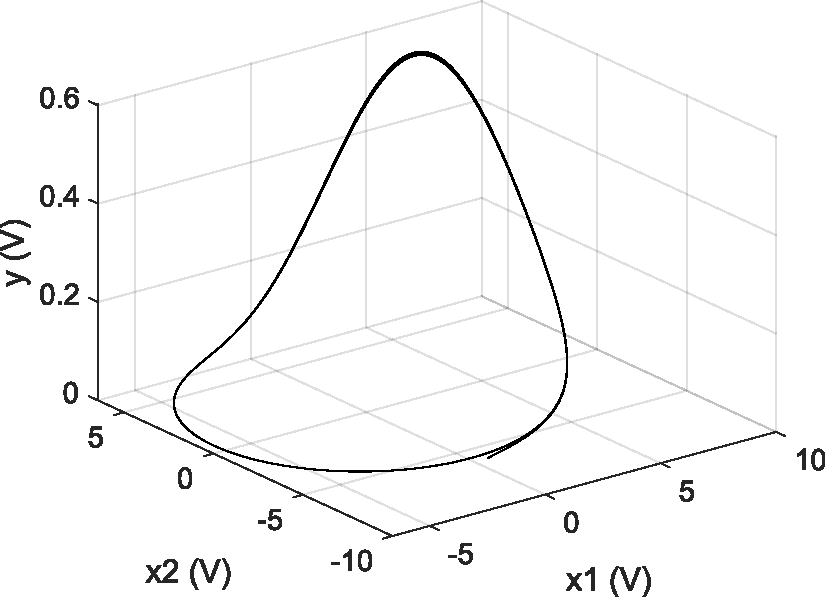
\includegraphics[scale=0.28]{figs/paraA/3dParaA3652.pdf}
            \caption{$R_{a_4} = 3652k\Omega$}   
            \label{fig:3dparaAvard}
        \end{subfigure}
        \caption{3D results for increments in $R_a$.} 
        \label{fig:3dparaAvar}
	\end{figure*}
	
	    \begin{figure*}
        \centering
        \begin{subfigure}[b]{0.22\textwidth}
            \centering
            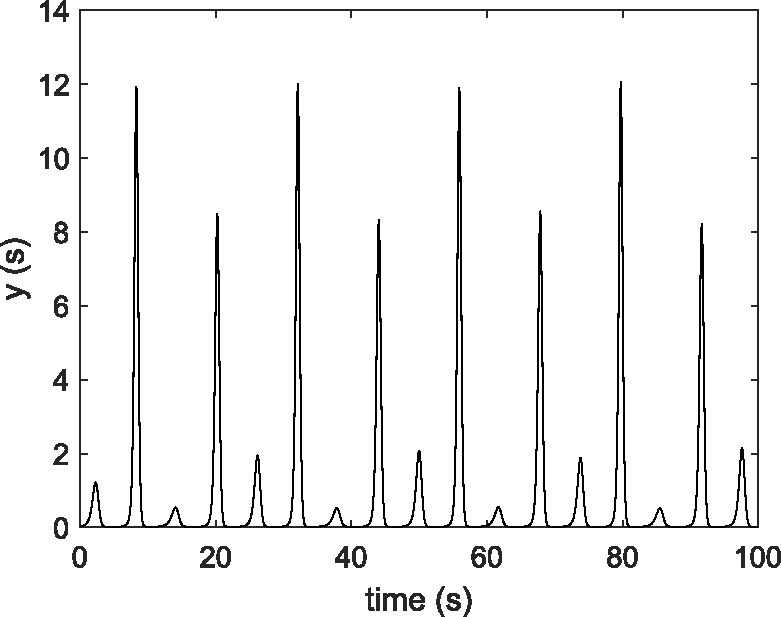
\includegraphics[scale=0.28]{figs/paraA/outParaA650.pdf}
            \caption{$R_{a_1} = 650k\Omega$.}    
        \end{subfigure}
        \begin{subfigure}[b]{0.22\textwidth}  
            \centering 
            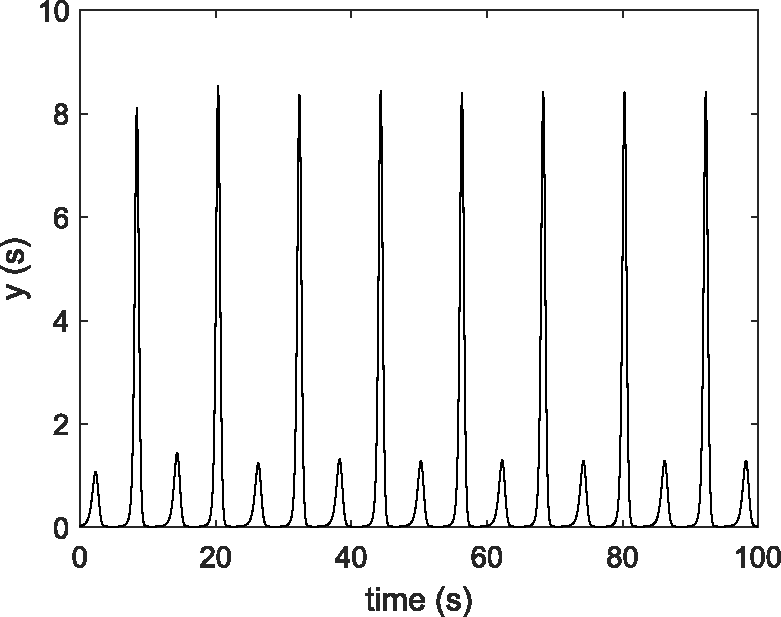
\includegraphics[scale=0.28]{figs/paraA/outParaA750.pdf}
            \caption{$R_{a_2} = 750k\Omega$.}  
        \end{subfigure}
        \begin{subfigure}[b]{0.22\textwidth}   
            \centering 
            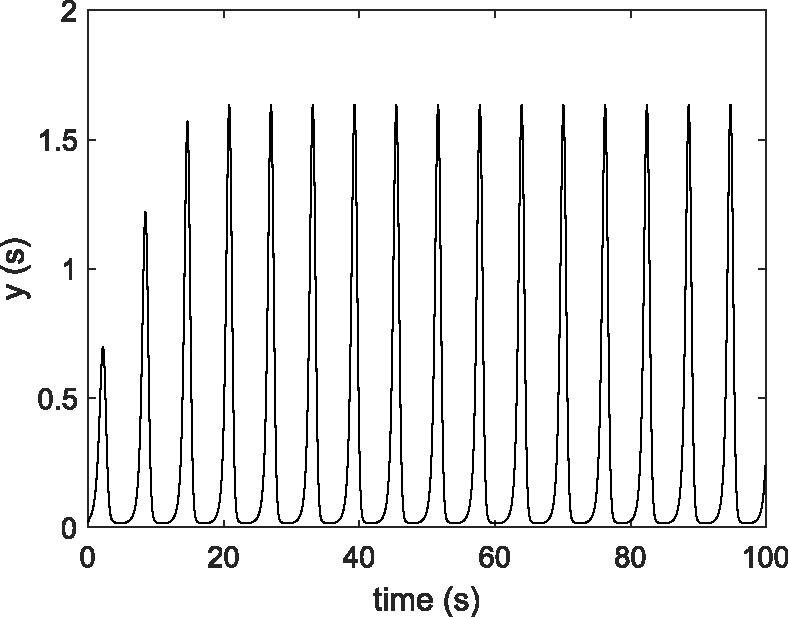
\includegraphics[scale=0.28]{figs/paraA/outParaA1750.pdf}
            \caption{$R_{a_3} = 1750k\Omega$}    
        \end{subfigure}
        \begin{subfigure}[b]{0.22\textwidth}   
            \centering 
            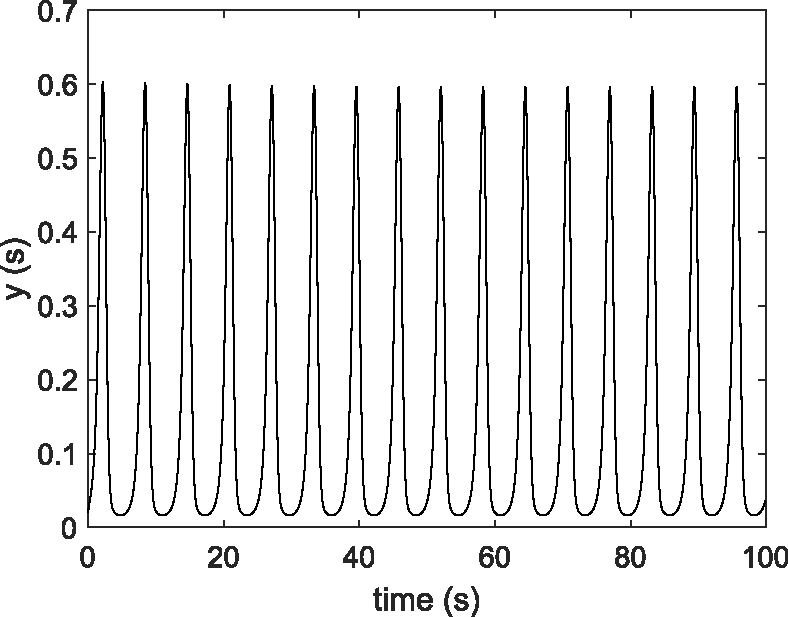
\includegraphics[scale=0.28]{figs/paraA/outParaA3652.pdf}
            \caption{$R_{a_4} = 3652k\Omega$}   
        \end{subfigure}
        \caption{Output signal in time for increments in $R_a$} 
        \label{fig:paraAvar}
	\end{figure*}
    
    \subsubsection{Parameter \texorpdfstring{$R_c$}{Rc}}\label{subsubsec:varparaC}
    Following the procedure of the previous section, both increments and smaller values of $R_c$ have been selected to evidence the response of the system. For the smaller values $R_{c_1}=10k\Omega$, $R_{c_2}=5k\Omega$, $R_{c_3}=2k\Omega$ and $R_{c_4}=1k\Omega$ have been selected. The results for the simulations with this parameters are shown in Figs. \ref{fig:3dparaCvarDown} and \ref{fig:paraCvarDown}.
    \begin{figure*}
        \centering
        \begin{subfigure}[b]{0.22\textwidth}
            \centering
            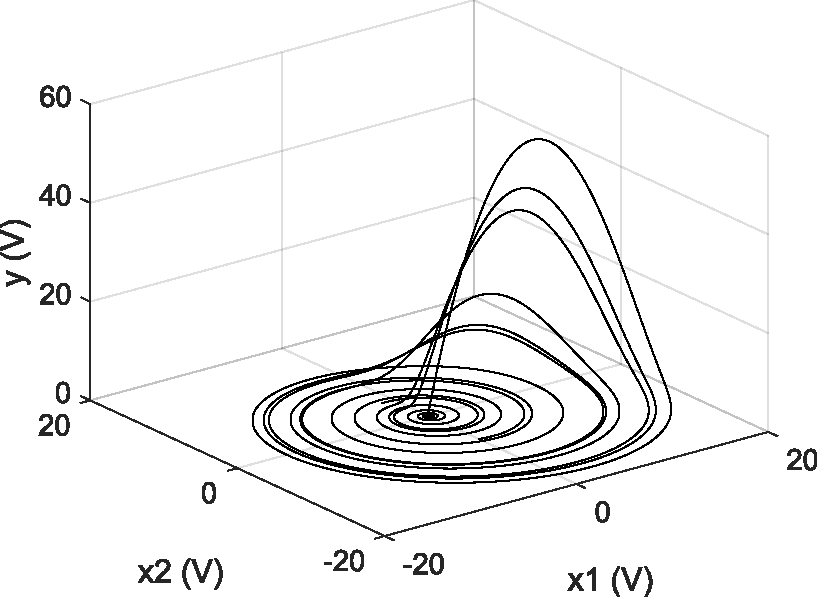
\includegraphics[scale=0.28]{figs/paraCdown/3dParaC10.pdf}
            \caption{$R_{c_1} = 10k\Omega$.}    
        \end{subfigure}
        \begin{subfigure}[b]{0.22\textwidth}  
            \centering 
            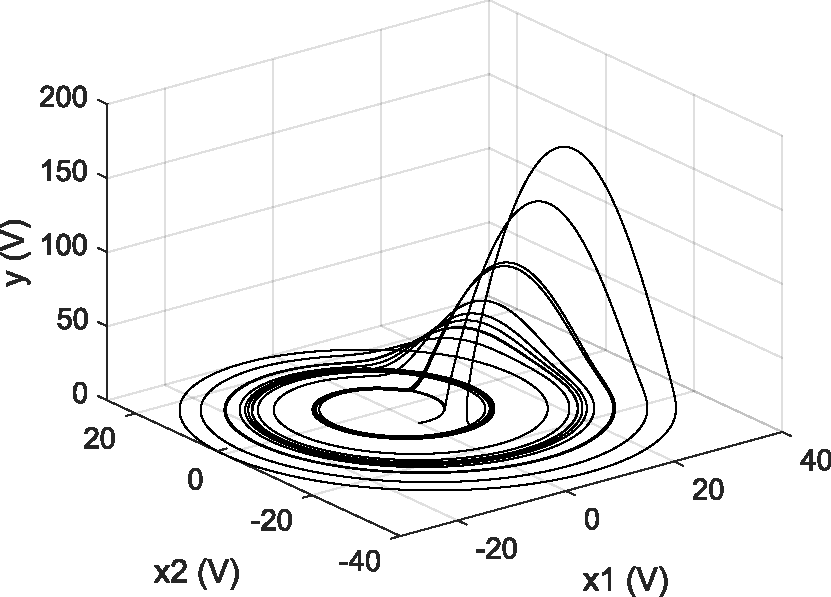
\includegraphics[scale=0.28]{figs/paraCdown/3dParaC5.pdf}
            \caption{$R_{c_2} = 5k\Omega$.}  
        \end{subfigure}
        \begin{subfigure}[b]{0.22\textwidth}   
            \centering 
            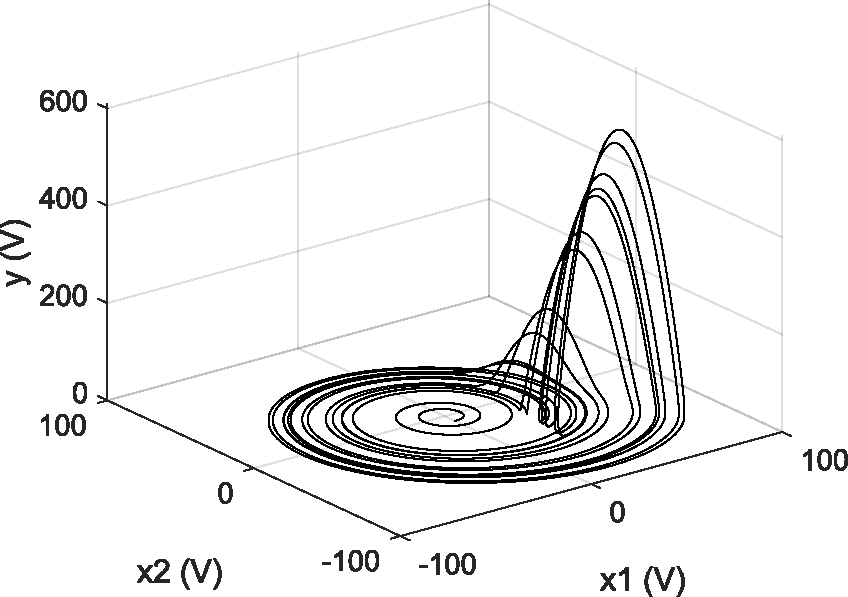
\includegraphics[scale=0.28]{figs/paraCdown/3dParaC2.pdf}
            \caption{$R_{c_3} = 2k\Omega$}    
        \end{subfigure}
        \begin{subfigure}[b]{0.22\textwidth}   
            \centering 
            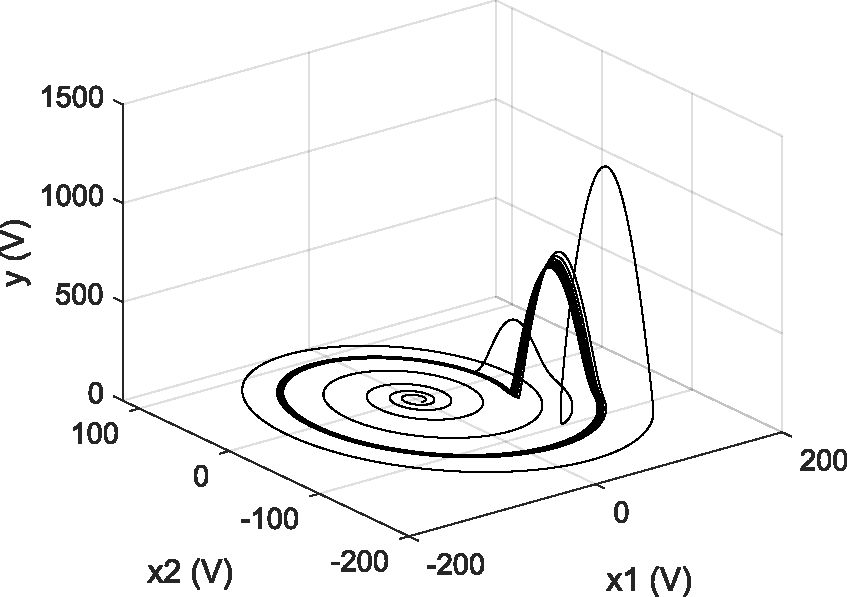
\includegraphics[scale=0.28]{figs/paraCdown/3dParaC1.pdf}
            \caption{$R_{c_4} = 1k\Omega$}
        \end{subfigure}
        \caption{3D results for smaller values of $R_c$.} 
        \label{fig:3dparaCvarDown}
	\end{figure*}
	
	    \begin{figure*}
        \centering
        \begin{subfigure}[b]{0.22\textwidth}
            \centering
            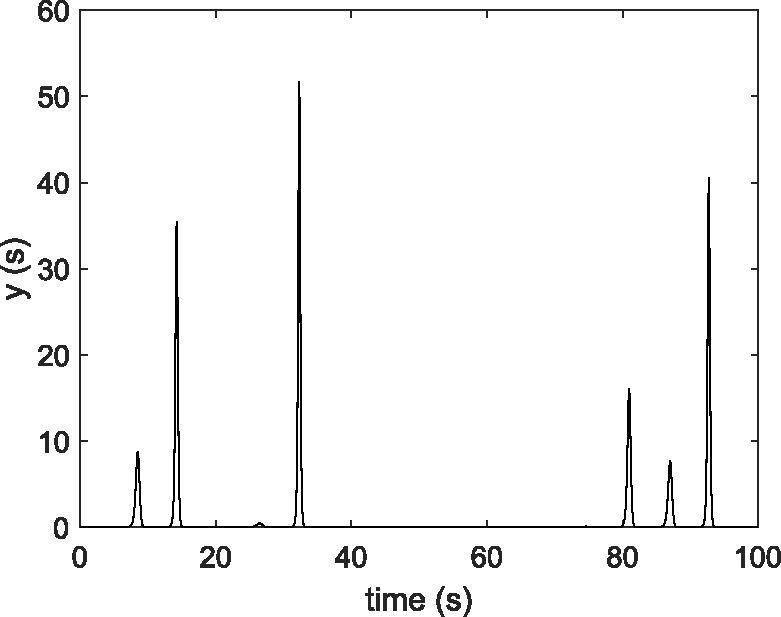
\includegraphics[scale=0.28]{figs/paraCdown/outParaC10.pdf}
            \caption{$R_{c_1} = 10k\Omega$.}    
        \end{subfigure}
        \begin{subfigure}[b]{0.22\textwidth}  
            \centering 
            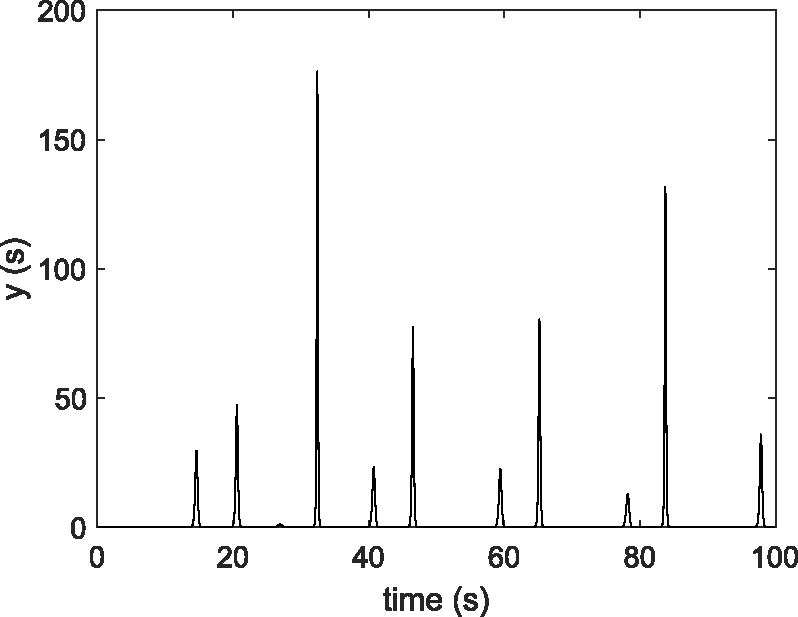
\includegraphics[scale=0.28]{figs/paraCdown/outParaC5.pdf}
            \caption{$R_{c_2} = 5k\Omega$.}  
        \end{subfigure}
        \begin{subfigure}[b]{0.22\textwidth}
            \centering 
            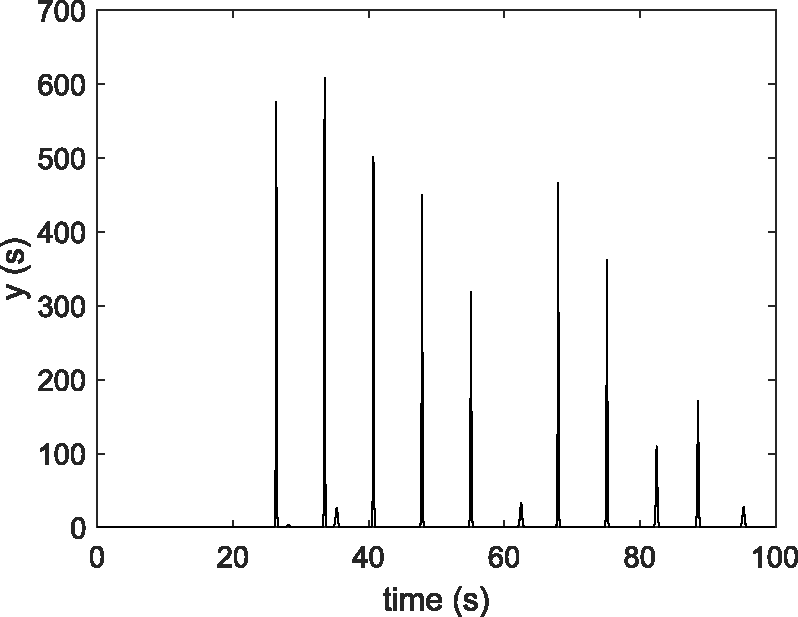
\includegraphics[scale=0.28]{figs/paraCdown/outParaC2.pdf}
            \caption{$R_{c_3} = 2k\Omega$}    
        \end{subfigure}
        \begin{subfigure}[b]{0.22\textwidth}   
            \centering 
            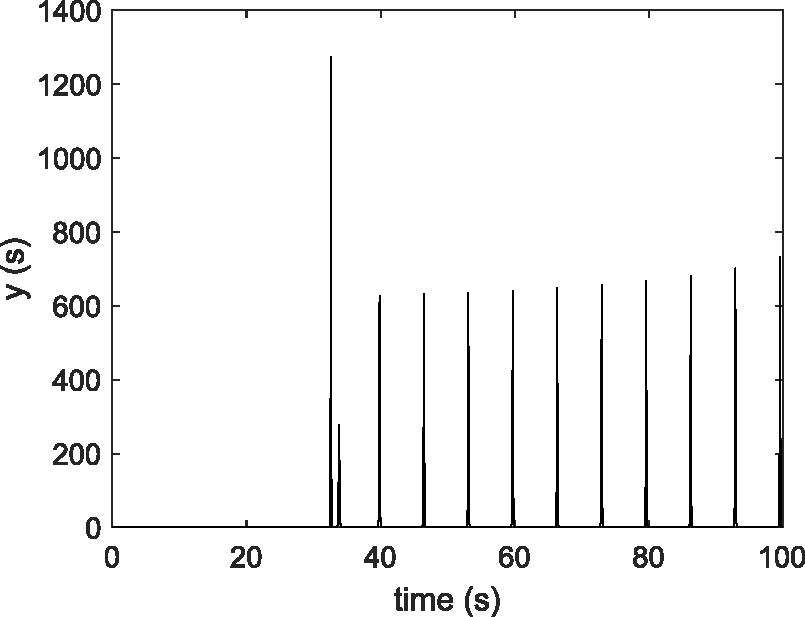
\includegraphics[scale=0.28]{figs/paraCdown/outParaC1.pdf}
            \caption{$R_{c_4} = 1k\Omega$}   
        \end{subfigure}
        \caption{Output signal in time for smaller values of $R_c$} 
        \label{fig:paraCvarDown}
	\end{figure*}
	
	For greater values, $R_{c_5}=10k\Omega$, $R_{c_6}=5k\Omega$, $R_{c_7}=2k\Omega$ and $R_{c_8}=1k\Omega$ were selected. The simulation results are shown in Figs. \ref{fig:3dparaCvarUp} and \ref{fig:paraCvarUp}.
	
	\begin{figure*}
        \centering
        \begin{subfigure}[b]{0.22\textwidth}
            \centering
            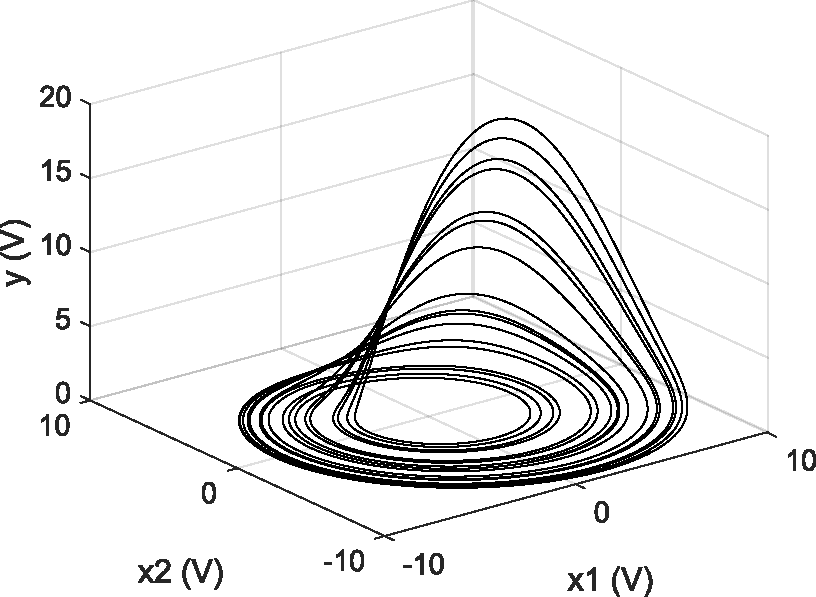
\includegraphics[scale=0.28]{figs/paraCup/3dParaC20.pdf}
            \caption{$R_{c_5} = 20k\Omega$.}    
        \end{subfigure}
        \begin{subfigure}[b]{0.22\textwidth}  
            \centering 
            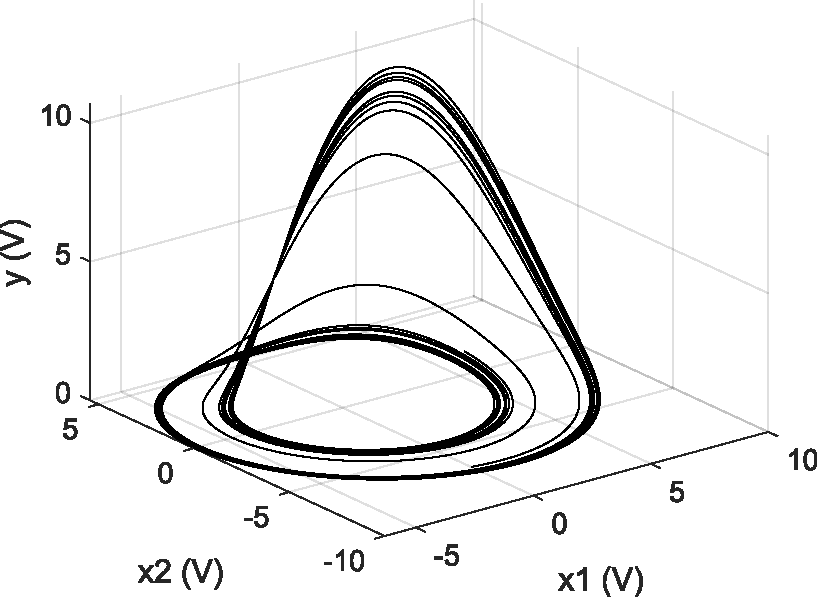
\includegraphics[scale=0.28]{figs/paraCup/3dParaC25.pdf}
            \caption{$R_{c_7} = 25k\Omega$.}  
        \end{subfigure}
        \begin{subfigure}[b]{0.22\textwidth}   
            \centering 
            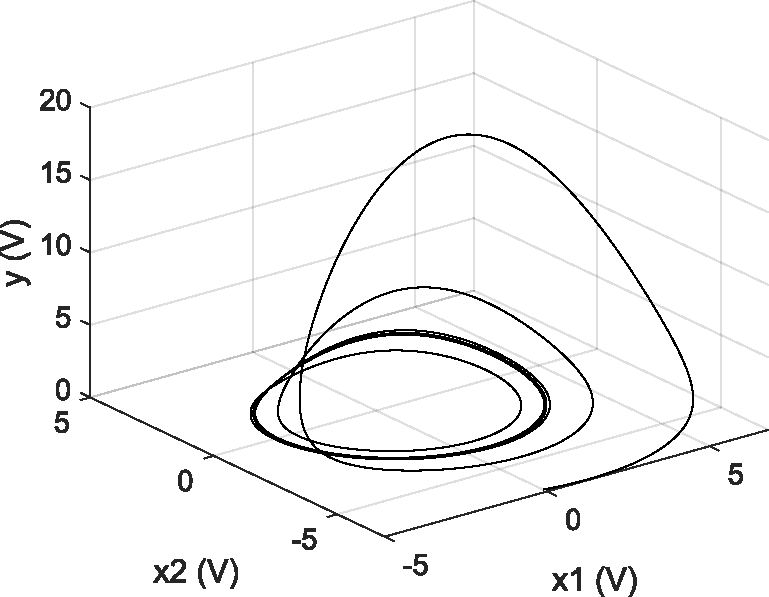
\includegraphics[scale=0.28]{figs/paraCup/3dParaC50.pdf}
            \caption{$R_{c_7} = 50k\Omega$}    
        \end{subfigure}
        \begin{subfigure}[b]{0.22\textwidth}   
            \centering 
            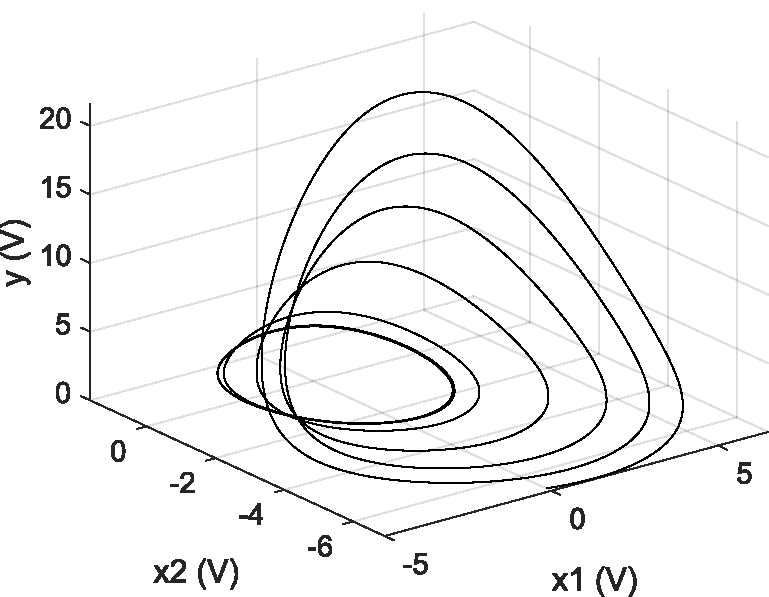
\includegraphics[scale=0.28]{figs/paraCup/3dParaC75.pdf}
            \caption{$R_{c_8} = 75k\Omega$}   
        \end{subfigure}
        \caption{3D results for increments in $R_c$.} 
        \label{fig:3dparaCvarUp}
	\end{figure*}
	
	    \begin{figure*}
        \centering
        \begin{subfigure}[b]{0.22\textwidth}
            \centering
            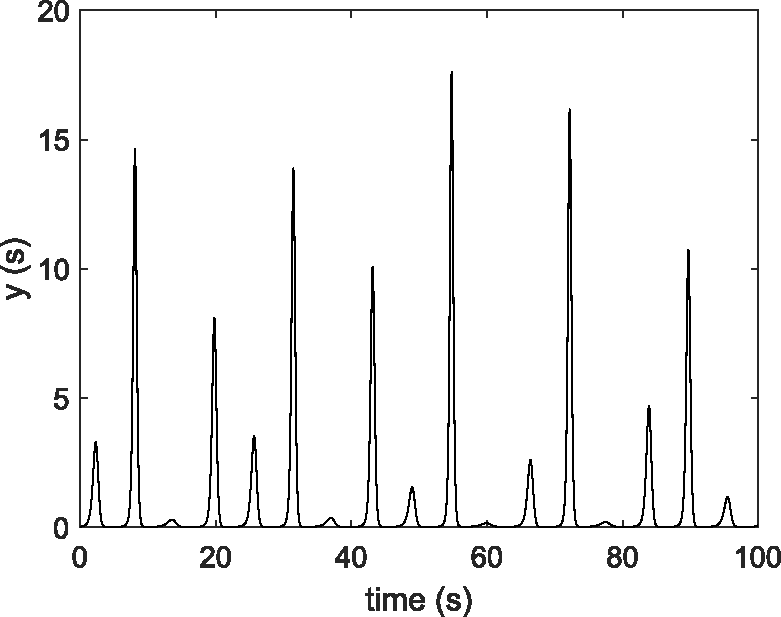
\includegraphics[scale=0.28]{figs/paraCup/outParaC20.pdf}
            \caption{$R_{c_5} = 20k\Omega$.}    
        \end{subfigure}
        \begin{subfigure}[b]{0.22\textwidth}  
            \centering 
            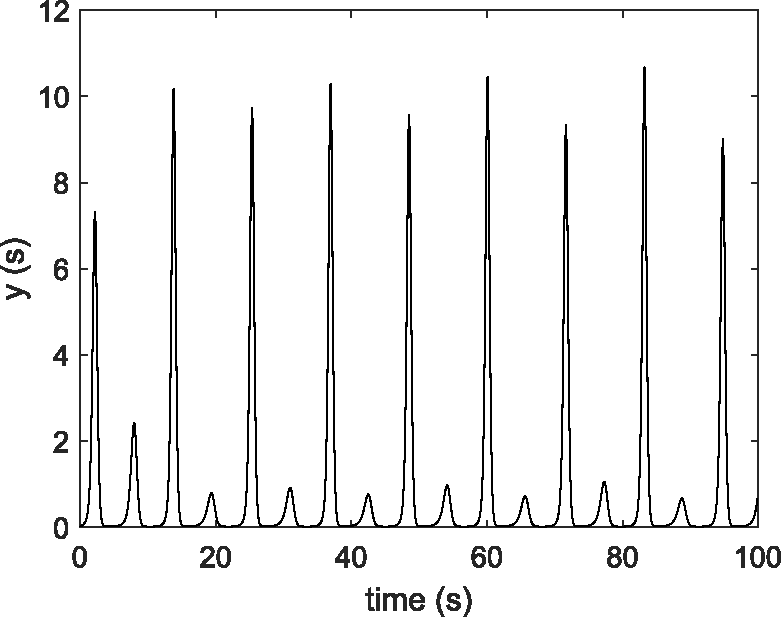
\includegraphics[scale=0.28]{figs/paraCup/outParaC25.pdf}
            \caption{$R_{c_6} = 25k\Omega$.}  
        \end{subfigure}
        \begin{subfigure}[b]{0.22\textwidth}   
            \centering 
            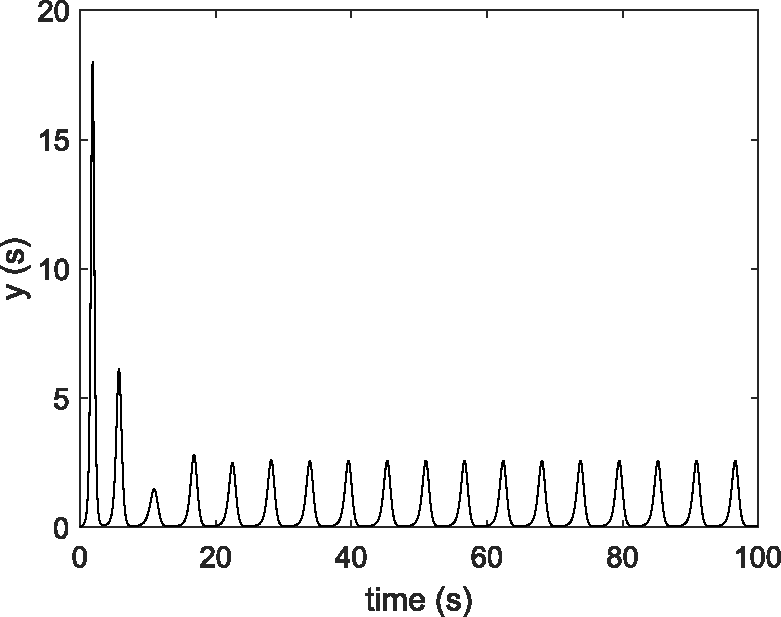
\includegraphics[scale=0.28]{figs/paraCup/outParaC50.pdf}
            \caption{$R_{c_7} = 50k\Omega$}    
        \end{subfigure}
        \begin{subfigure}[b]{0.22\textwidth}
            \centering 
            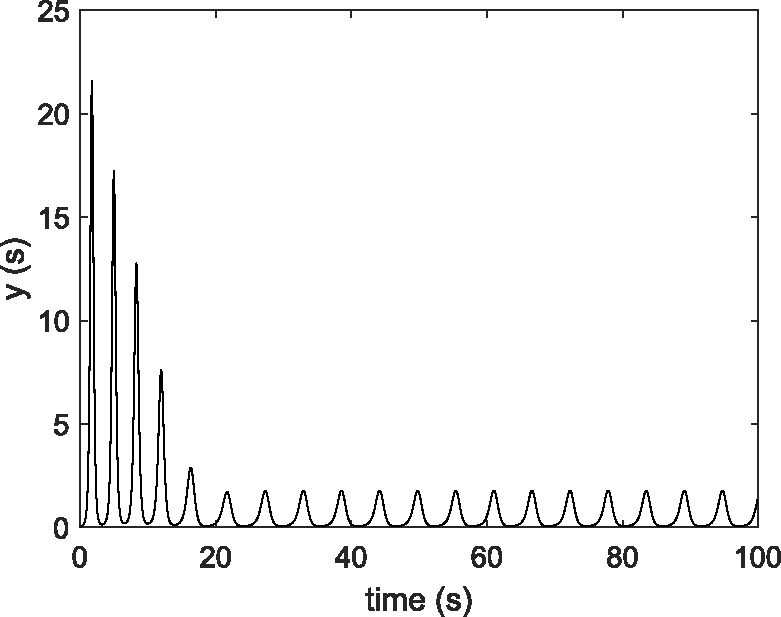
\includegraphics[scale=0.28]{figs/paraCup/outParaC75.pdf}
            \caption{$R_{c_8} = 75k\Omega$}  
            \label{fig:paraCvarUpd}
        \end{subfigure}
        \caption{Output signal in time for increments in $R_c$} 
        \label{fig:paraCvarUp}
	\end{figure*}
	
    %%%%%%%%%%%%%%%%%%%%%%%%%%%%%%%%%%%%%%%%%%%%%%%%%%%%%%%%%%%%%%%%%%%%%%%%%%%%%%
    \subsection{Limit for Parameter Variation}
    In the following simulations, extreme values for $R_a$ and $R_c$ are presented; that is, values for which the output $y$ starts to behave unaccordigly. The values presented here were found following a bisection method, between a known normal behavior for the system and a point where the derivative in the simulation was not finite.
    
    \subsubsection{Parameter \texorpdfstring{$R_a$}{Ra}}\label{subsubsec:ra}
    First, a significantly close value to the minimum for $R_a$ was obtained around $259.098131084k\Omega$. In Figs. \ref{fig:outParaAdown} and \ref{fig:3dParaAdown} the behavior of the output in time and all three variables is shown.
    \begin{figure}[H]
        \centering
        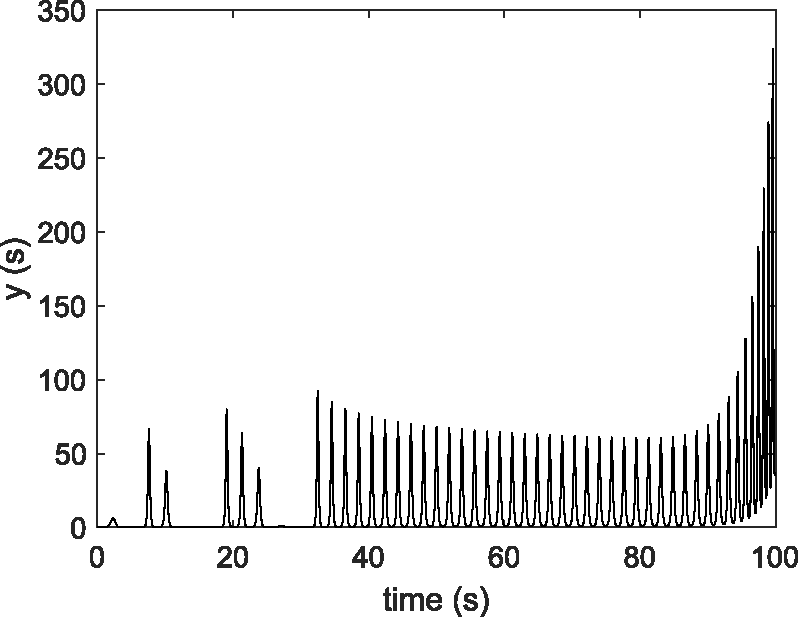
\includegraphics[scale=0.5]{figs/outParaAdown.pdf}
        \caption{Output signal in significant time for reduction in parameter $R_a$.}
        \label{fig:outParaAdown}
    \end{figure}
    \begin{figure}[H]
        \centering
        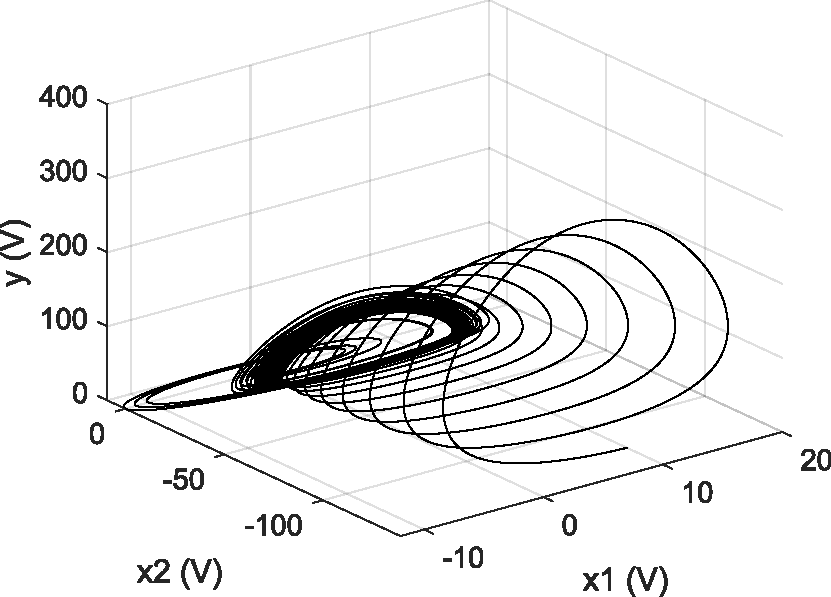
\includegraphics[scale=0.5]{figs/3dParaAdown.pdf}
        \caption{3D phase plot for the state variables for a significant reduction in parameter $R_a$.}
        \label{fig:3dParaAdown}
    \end{figure}
    
     Notice that, in the three-dimensional plot for the state variables, the trajectory starts to separate from the attractor; in the graph of $y$ against time, the output signal explodes and as $t$ increases, the output tends to infinity.
    
    Second, $R_a$ was set to $10000k\Omega$; this value was not found with the bisection method, since $R_a$ can take arbitrarily large numbers and all show the same output. In Figs. \ref{fig:outParaAup} and \ref{fig:3dParaAup} the behavior of the output in time and all three variables is shown.
    \begin{figure}[H]
        \centering
        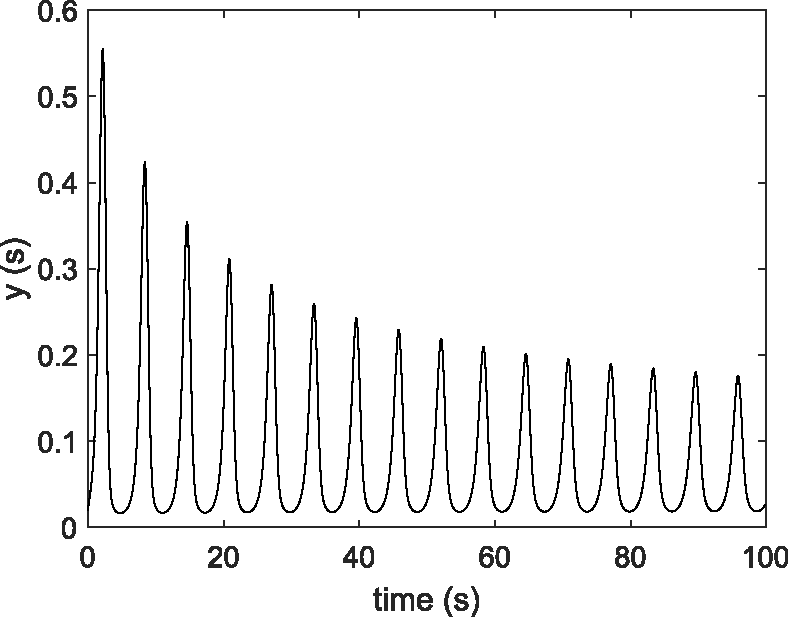
\includegraphics[scale=0.5]{figs/outParaAup.pdf}
        \caption{Output signal in time for a significant increment in parameter $R_a$.}
        \label{fig:outParaAup}
    \end{figure}
    \begin{figure}[H]
        \centering
        \includegraphics[scale=0.5]{figs/3dParaAup.pdf}
        \caption{3D phase plot for the state variables for an increment in parameter $R_a$.}
        \label{fig:3dParaAup}
    \end{figure}
    
    For the increment of $R_a$, the system behavior is periodic bounded by a decreasing signal, as the plot of $y$ against time shows. The 3D plots shows that the orbit falls into a decreasing loop.
    
    \subsubsection{Parameter \texorpdfstring{$R_c$}{Rc}}
    Following the idea from section \ref{subsubsec:ra}, the found minimum found value for $R_c$ is around $0.08400331675k\Omega$. In Figs. \ref{fig:outParaCdown} and \ref{fig:3dParaCdown} the behavior of the output in time and all three variables is shown.
    \begin{figure}[H]
        \centering
        \includegraphics[scale=0.5]{figs/outParaCdown.pdf}
        \caption{Output signal in significant time for reduction in parameter $R_c$.}
        \label{fig:outParaCdown}
    \end{figure}
    \begin{figure}[H]
        \centering
        \includegraphics[scale=0.5]{figs/3dParaCdown.pdf}
        \caption{3D phase plot for the state variables for a significant reduction in parameter $R_c$.}
        \label{fig:3dParaCdown}
    \end{figure}
    
    Notice that, in the 3D plot, the opening of the attractor is shrinked, compared to higher values for $R_c$. The peaks in the output signal are much bigger than the standard values (order of $10^{4}$).
    
    For the increment maximum value in $R_c$, around $88.48868k\Omega$ was found with the bisection method. In Figs. \ref{fig:outParaCup} and \ref{fig:3dParaCup} the behavior of the output in time and all three variables is shown.
    \begin{figure}[H]
        \centering
        \includegraphics[scale=0.5]{figs/outParaCup.pdf}
        \caption{Output signal in time for a significant increment in parameter $R_c$.}
        \label{fig:outParaCup}
    \end{figure}
    \begin{figure}[H]
        \centering
        \includegraphics[scale=0.5]{figs/3dParaCup.pdf}
        \caption{3D phase plot for the state variables for an increment in parameter $R_c$.}
        \label{fig:3dParaCup}
    \end{figure}
    
    \subsection{Euler and Runge-Kutta Methods}\label{subsec:methods}
    A short comparison between the numerical methods was done, running simulations using Simulink's integrated methods and the manually programmed methods in Matlab for both fourth-order Runge-Kutta and Euler's method. The results are shown in Fig. \ref{fig:MethodMethod}.
    \begin{figure}[H]
        \centering
        \begin{subfigure}[b]{0.475\textwidth}
            \centering
            \includegraphics[scale=0.5]{figs/EulerEuler.pdf}
            \caption{}
        \end{subfigure}
        \vskip\baselineskip
        \begin{subfigure}[b]{0.475\textwidth}   
            \centering 
            \includegraphics[scale=0.5]{figs/RungeRunge.pdf}
            \caption{}
        \end{subfigure}
        \caption{System simulation with both Runge-Kutta and Euler methods using Simulink and programming the difference equation.}
        \label{fig:MethodMethod}
	\end{figure}

\section{Results analysis}\label{sec:resultAn}
%%%%%%%%%%%%%%%%%%%%%%%%%%%%%%%%%%%%%%%%%%%%%%%%%%%%%%%%%%%%%%%
\subsection{Comparison between the Linear and Nonlinear Systems}
As it has been mentioned before, the linearization of the Rössler system (\ref{eq:state}) was performed based on previous results in \cite{JS_PL}; there, it was found that the Rössler system is completely stable for large inputs, around $1000V$. Therefore, the equilibrium points were calculated based on this input and the linear model was obtained.

The linearity curve, discussed in section \ref{sec:linearityCurve} and presented in Fig. \ref{fig:linearityCurve}, was developed in order to see where the linear system can successfully reach the same stationary state as the nonlinear. From the linearity curve, the linearity interval can also be extracted: in the curve, it can be observed that both systems (in stationary state) are really close from one another for $u$ between $0V$ to $250V$. This means that the systems have the almost the same stationary state for inputs $u\in[0V,250V]$, and this can also be verified in the simulations performed.

In section \ref{sec:compar_LinearNonlinear}, the inputs were chosen according to the linearity curve. Recall Fig. \ref{fig:comparDelta0}, note that both systems do not present changes in the output and they completely overlap; this is caused by the input selected: $1000V$. Since both systems are exactly at the operation point, which was chosen as an equilibrium point, their states do not change over time. In the next simulation, $1050V$ was selected as input; Fig. \ref{fig:comparDelta50} shows the responses to this input, note that they present almost the exact same behavior, only differing in the peaks and valleys of the oscillation only by a really small factor. This can be partially explained with the linearity curve: both systems are equal in stationary state. The linearity curve does not provide information about the transitory state but as the input selected was chosen near to the operation point, both systems present equal behavior in transitory state as well.

In Fig. \ref{fig:comparDelta200}, the responses are shown for an input of $1200V$. Note that they start to differ a little bit, but it is still a value inside the range of linearity, that is why the stationary state is close. It is important to highlight that the transitory state of the linear approximation is not too different from the nonlinear one, they present similar behavior and same oscillation frequency; it can be observed that the Rössler system present larger damping, as it stabilizes faster than the linear approximation. Finally, in Fig. \ref{fig:comparDelta750}, the responses of the systems are displayed, but for an input outside of the linearity range ($1750V$). As expected, the systems stabilize in different values, but the linear system does a good approximation at the start of the simulation, but couldn't reproduce the strange and quick stabilization of the nonlinear system. The last graph (Fig. \ref{fig:sinInput_compar}) shows the output for both systems to a sine input; since the linear system can successfully represent the nonlinear Rössler, for inputs close to the operation point, it was expected that the output for the nonlinear system would be a sine wave as well and, as this figure shows, the output was exactly the same. This is due to the sine wave chosen: as the amplitude is so small compared with the linearity range, all the values that the sine input take are contained in the linearity interval.

For a comparison in regarding the initial conditions, section \ref{sec:initCondCompar}, the initial conditions for the output state $x_3$ were changed. For a really small change $\varepsilon=0.1V$ and a medium change $\varepsilon=50V$, the system is stable and its state returns to the equilibrium point; this yields that the operation point chosen is an stable equilibrium point (at least in $x_3$) since the nonlinear system, for small changes in the initial conditions, it returns over time to the same equilibrium point, as it is shown in Figs. \ref{fig:ci_x3_01} and \ref{fig:ci_x3_50}, even though their transitory state differ. The next simulation was performed with $\varepsilon=400V$, which is significantly far from the operation point; in Fig. \ref{fig:ci_x3_400}, the responses were presented; notice that the nonlinear system starts to diverge from the operation point; the reason for this is explained by the nonlinear dynamics associated with the Rössler system: it is likely that the system is going to another equilibrium point or just growing unboundedly, or it will start to show strange attractor properties and chaos.

One last comparison was developed with small and medium changes in the initial conditions and the input. From Fig. \ref{fig:Delta_all_small}, the response of both systems in shown; as the input selected ($1003V$) is so close to the operation point (and in the linearity range) and as the changes in the initial conditions are so subtle (stable operation point), both systems will show exactly the same behavior. On the other hand, as it can be observed in Fig. \ref{fig:Delta_all_large}, the nonlinear system shows a strange transitory state that clearly cannot be obtained with the linear approximation; although, both systems stabilize in the same equilibrium point.

%%%%%%%%%%%%%%%%%%%%%%%%%%%%%%%%%%%%%%%%%%%%%%%%%%%%%%%%%%%%%%%
\subsection{Continuous and Discrete Transfer function}
In section \ref{sec:tf}, the continuous transfer function was found. This function has some important properties to notice; in first place, it represents a non-minimum phase system as the zeros, found in \ref{sec:order_reduction}, have a positive real part. This is really noticeable in Fig. \ref{fig:growth_Time} where when the system is reaching its maximum value, instead of growing constantly to the peak it decreases for a moment and then proceeds to keep growing. On the other hand, it is confirmed that the system is stable as all the poles have negative real part.

For the sample time selection, it was specially important that the discretization does not lose main properties of the system; specially, the non-minimum phase property discussed before. As seen in Fig. \ref{fig:tfsStep}, from the discrete system the original signal could be reconstructed without losing too much information about it. Note that even if the sample time selection was selected using a different simulation, for Fig. \ref{fig:tfsImpulse}, the sample time is also a sufficient value to be able to reconstruct the signal without losing too much information. 

It is important to analyze why is there an existence of a lower bound for the sample time, if a big selection could generate problems, such as aliasing. This is explained as, if it was chosen to be indefinitely small, it would be impossible to keep sampling the output in an experiment, as a really low sampling time cannot be replicated easily; also, the discrete signal would almost be continuous therefore, losing its purpose of making the signal discrete.

Additionally, about the response found in Fig. \ref{fig:tfsStep} and Fig. \ref{fig:tfsImpulse}, it is important to notice how, in the first one, it stabilized in other place different from the initial conditions as the input was a constant step that made the system increase it's energy. On the other hand, when the impulse was given to the system in the second figure, it gain a high momentum for a bit and then comes back to the initial point, as the input goes to zero as soon as it transfers that momentum to the system.

Lastly, the discrete ponderation sequence is verified as every point calculated using it overlaps the continuous graph. It was noticed that this weighting sequence is really useful, as the convolution product is an easy operation to calculate and inverse zeta transform would be only used one time instead of using it every time it is needed to simulate with a different input.

In conclusion, the transfer function is a useful tool for simulating and saving the information about a linear system with null initial conditions specially for a SISO system.

%%%%%%%%%%%%%%%%%%%%%%%%%%%%%%%%%%%%%%%%%%%%%%%%%%%%%%%%%%%%%%%
\subsection{Order reduction}
In first place, it is seen that the \textit{Matlab} reduction and the elimination of an insignificant pole are barely different as seen in equation \ref{eq:reduced_matlab} and \ref{eq:reduced_insignificant}. This happens because the software used utilizes numerical algorithms to find a fitting reduction for the system; instead, the other one was using analytical methods which would have more precision. In this manner, it is assured that both models are the same. Furthermore, if Fig. \ref{fig:reduced_matlab} and Fig. \ref{fig:reduced_insignificant} are compared this thesis is confirmed even more, as the minor differences between the two plots can be explained by the same numerical errors.

In second place, there is an apparent contradiction that occurs in Fig. \ref{fig:reduced_insignificant}. It occurs, apparently, that the initial conditions of the system simulated are not 0, as it is seen in the comparison between the reduced system and the original system. This happens due to the obtained transfer function is strictly proper therefore, by the initial value theorem, the output would have a not null initial condition. Although this is a good reason why this occurs it is still an incomplete view of the problem.

In third place, the approximated approach did exactly what the system was purposed of as both systems have the same growth time, stationary state and maximum peak. On the other hand, the approximated approach does not take into account the non-minimum property as that system has not finite zeros; therefore, in the graph it grows continuously instead of taking a slight step backwards as in the original system. This behaviour, although not very representative of the original system, it is desirable as it would represent a causal system; in this manner, this reduced system is preferable than the others if the circuit is going to be recreated experimentally.

In conclusion, there was found two different models (the \textit{Matlab} reduction and analytic one are considered the same as explained before) that represent the system to a certain degree of lower order than the original linear Rössler system.. The analytic system, ensures to represent the system in it's transitory state and final state except at the start in which it changes the initial conditions; the approximated approach was close to the system in it's final state and peak but not during it's transitory state but, it is more practical to use in real life as this reduced system is minimum phase.

%%%%%%%%%%%%%%%%%%%%%%%%%%%%%%%%%%%%%%%%%%%%%%%%%%%%%%%%%%%%%%%
\subsection{Stability Analysis}
The parameter $R_a$, chosen to make the stability analysis has no special properties; the same procedure could have been made for parameter $R_c$ or $RC$. As presented in section \ref{sec:order_reduction}, all the poles of the linearized Rössler system satisfy $\Re(\lambda_i)<0$, therefore the system is stable; from the simulations performed in \ref{sec:compar_LinearNonlinear}, it can also be proved, graphically, that the system is stable.

It was desired to analyze for which values of $R_a$, the linear system is stable; in order to achieve this, it was required to obtain the characteristic polynomial in terms of $R_a$, since the roots of this polynomial are the poles of the linear system. This polynomial, presented in equation (\ref{eq:charPoly}), will have all their roots in the left half-plane when the Routh-Hurwitz necessary and sufficient conditions are satisfied. This process lead to the condition $R_a>184.7341k\Omega$; this implies that the resistor $R_a$ can take values greater than this condition and the linear system will be stable. This is presented as well with the simulations performed, showed in Fig. \ref{fig:Ra_Dentro}a); as expected, the linear system is stable. On the other hand, for the stability of the nonlinear system, it would be necessary to make a deeper analysis, with Lyapunov theory for example; although, the simulations performed and showed in \ref{fig:Ra_Dentro}b) proves that the nonlinear system is stable for $184k\Omega\leq R_a\leq300k\Omega$. It could be also proposed that the Rössler system 

In Fig. \ref{fig:Ra_Fuera}a), the results of the linear system for values of $R_a$ outside the stability region found are presented, this is another validation of the region found. Another important annotation is that the nonlinear system still has stable values outside the region of stability for the linear model, again, since the nonlinear system requires much further study; notice in Fig. \ref{fig:Ra_Fuera}b) that the nonlinear system is still stable for $R_a\geq170k\Omega$. Hence, it can be asserted that the Rössler system in study is stable for $170k\Omega\leq R_a\leq300k\Omega$, which is an important property that had to be mentioned.

All the previous analysis could have been performed with the root locus method, recall Fig. \ref{fig:root_locus}, remember that the root locus starts in the poles and ends in the zeros of the associated transfer function for the parameter in study, as depicted in \ref{sec:root_locus}. The poles are marked with an $\times$ and the zeros with a $\circ$. Note that one root make almost no movement for $k\geq0$ but is in the left half-plane; one of the other two roots starts in the left half-plane as well, whereas the other one start in the right half-plane in $+\infty$, but this plot also shows that there exists some values of $R_a$ that stabilize the system; note that, after the roots reach the break point, both of them start moving towards the left half-plane and actually crossing into it towards the ``end'' of their trajectories, making all of the characteristic polynomial roots satisfy $\Re(\lambda_i)<0$.

%%%%%%%%%%%%%%%%%%%%%%%%%%%%%%%%%%%%%%%%%%%%%%%%%%%%%%%%%%%%%%%
\subsection{Bode Diagram}
Firstly, yet again it is confirmed that the linear system is non-minimum phase. This happens because, if it would, then the change of phase of the bode diagram would be -180° instead of -360° as seen in Fig. \ref{fig:contBode}. It is commonly said that for non-minimum phase systems the bode diagram is not a good tool for representing the original system as it gives wrong information; in this manner, it is said in the literature, that the Nyquist diagram is more useful. On the other hand, in our testing the bode diagram gave correct information about the original system.

Furthermore, in Fig. \ref{fig:bodePoints}, it can be seen that for an sine wave input with a frequency of $\omega = 1 rad/s$ the system would have decibels magnitude of -55.5. Using the formulas explained in methods, the stationary state would be given by the wave in equation \ref{eq:sine_ss}. So, the system was simulated with this conditions and as seen in Fig. \ref{fig:bode_sineOutput}, the stationary state matches almost perfectly with the sine wave predicted by the bode diagram. In this manner, the small discrepancies between both simulations can be due to small numerical errors made by the software.

In second place, the discrete bode diagram does have the expected behaviour as it is very similar to the continuous one until it starts approach the Nyquist frequency which, start distorting the original signal so it starts not giving reliable information. Although there was not any simulation performed using this information, it is argued that because the similar behaviour of the discrete bode diagram to the continuous one it is confirmed that it does represent the original system at least for frequencies much smaller than the Nyquist one.

In third place, for the reduced model it is important to notice that the valley encountered at $\omega = 1 rad/s$ has the same magnitude as the one encountered in the original system. Therefore, for frequencies in that valley and before the reduced system is a very good approximation of the original system. On the other hand, for frequencies beyond this valley it would seem as the magnitude becomes constant again not representing at all the behaviour of the not reduced model. This happens because, when the model was reduced the transfer function became not strictly proper therefore, making it have a rate of change of 0; at the same time, this warns that if the reduced model is going to be used instead of the original system, for frequencies larger than $\omega = 2 rad/s$ the reduced model is useless to examine the original system.

In third place, for the closed-loop stability in the bode diagram it is seen that the phase plot does not cross the -180° value therefore it would seem as it did not had any crossover phase frequency. But, \textit{Matlab} presented a value for this property because, there are several distinct definitions to calculate the different margins of the system and instead of seeing when the phase plot crosses the value selected it could be analyzed, instead, for 180°. In this manner, this value for the $k_max$ was verified ins Fig. \ref{fig:response_gains_k} and Fig. \ref{fig:response_gains_unstable} in which inside and outside the stability region it behaves as it is predicted. 

On the other hand, for the unstable plot it would seem the first two values are critically stable instead of unstable; this happens because the growth of the value of the system is changing slightly, therefore it would be needed a lot more time to show this and it would be difficult to present the results in an organized way. Lastly, in Fig. \ref{fig:response_delays}, it was shown that for any delay chosen the system can not be unstabilized by this value.

In conclusion, the bode diagram was a useful tool which presented good information of the system when the input is a sine wave. This information allowed to calculate an interval for the stability of the closed loop system which was confirmed for the simulations presented.
\section{Conclusions}\label{sec:conc}
In this work, a linear control to the Rössler circuit proposed by \cite{canals2014random} was successfully designed with the procedures presented in section \ref{sec:meth}, and then tested under different conditions. Although, some approaches (Ziegler-Nichols and Chien-Hrones-Reswick) did not provide good approximations for the discrete PID controller, the sensitivity and analytic methods showed proper behavior for certain intervals of the inputs and the $R_a$ parameter, usually with an upper bound of $u_{ub} = 1.5$ and $R_a = 3000$, achieving absolute stability and eliminating steady-state error for a step and ramp input.

\nocite{*}
\bibliography{ref}
\bibliographystyle{IEEEtran}
\end{document}
